\documentclass[twoside]{book}

% Packages required by doxygen
\usepackage{fixltx2e}
\usepackage{calc}
\usepackage{doxygen}
\usepackage[export]{adjustbox} % also loads graphicx
\usepackage{graphicx}
\usepackage[utf8]{inputenc}
\usepackage{makeidx}
\usepackage{multicol}
\usepackage{multirow}
\PassOptionsToPackage{warn}{textcomp}
\usepackage{textcomp}
\usepackage[nointegrals]{wasysym}
\usepackage[table]{xcolor}

% Font selection
\usepackage[T1]{fontenc}
\usepackage[scaled=.90]{helvet}
\usepackage{courier}
\usepackage{amssymb}
\usepackage{sectsty}
\renewcommand{\familydefault}{\sfdefault}
\allsectionsfont{%
  \fontseries{bc}\selectfont%
  \color{darkgray}%
}
\renewcommand{\DoxyLabelFont}{%
  \fontseries{bc}\selectfont%
  \color{darkgray}%
}
\newcommand{\+}{\discretionary{\mbox{\scriptsize$\hookleftarrow$}}{}{}}

% Page & text layout
\usepackage{geometry}
\geometry{%
  a4paper,%
  top=2.5cm,%
  bottom=2.5cm,%
  left=2.5cm,%
  right=2.5cm%
}
\tolerance=750
\hfuzz=15pt
\hbadness=750
\setlength{\emergencystretch}{15pt}
\setlength{\parindent}{0cm}
\setlength{\parskip}{3ex plus 2ex minus 2ex}
\makeatletter
\renewcommand{\paragraph}{%
  \@startsection{paragraph}{4}{0ex}{-1.0ex}{1.0ex}{%
    \normalfont\normalsize\bfseries\SS@parafont%
  }%
}
\renewcommand{\subparagraph}{%
  \@startsection{subparagraph}{5}{0ex}{-1.0ex}{1.0ex}{%
    \normalfont\normalsize\bfseries\SS@subparafont%
  }%
}
\makeatother

% Headers & footers
\usepackage{fancyhdr}
\pagestyle{fancyplain}
\fancyhead[LE]{\fancyplain{}{\bfseries\thepage}}
\fancyhead[CE]{\fancyplain{}{}}
\fancyhead[RE]{\fancyplain{}{\bfseries\leftmark}}
\fancyhead[LO]{\fancyplain{}{\bfseries\rightmark}}
\fancyhead[CO]{\fancyplain{}{}}
\fancyhead[RO]{\fancyplain{}{\bfseries\thepage}}
\fancyfoot[LE]{\fancyplain{}{}}
\fancyfoot[CE]{\fancyplain{}{}}
\fancyfoot[RE]{\fancyplain{}{\bfseries\scriptsize Generated by Doxygen }}
\fancyfoot[LO]{\fancyplain{}{\bfseries\scriptsize Generated by Doxygen }}
\fancyfoot[CO]{\fancyplain{}{}}
\fancyfoot[RO]{\fancyplain{}{}}
\renewcommand{\footrulewidth}{0.4pt}
\renewcommand{\chaptermark}[1]{%
  \markboth{#1}{}%
}
\renewcommand{\sectionmark}[1]{%
  \markright{\thesection\ #1}%
}

% Indices & bibliography
\usepackage{natbib}
\usepackage[titles]{tocloft}
\setcounter{tocdepth}{3}
\setcounter{secnumdepth}{5}
\makeindex

% Custom commands
\newcommand{\clearemptydoublepage}{%
  \newpage{\pagestyle{empty}\cleardoublepage}%
}

\usepackage{caption}
\captionsetup{labelsep=space,justification=centering,font={bf},singlelinecheck=off,skip=4pt,position=top}

%===== C O N T E N T S =====

\begin{document}

% Titlepage & ToC
\pagenumbering{alph}
\begin{titlepage}
\vspace*{7cm}
\begin{center}%
{\Large elektrokardiograf }\\
\vspace*{1cm}
{\large Generated by Doxygen 1.8.14}\\
\end{center}
\end{titlepage}
\clearemptydoublepage
\pagenumbering{roman}
\tableofcontents
\clearemptydoublepage
\pagenumbering{arabic}

%--- Begin generated contents ---
\chapter{Hierarchical Index}
\section{Class Hierarchy}
This inheritance list is sorted roughly, but not completely, alphabetically\+:\begin{DoxyCompactList}
\item \contentsline{section}{Aparatmedyczny}{\pageref{class_aparatmedyczny}}{}
\begin{DoxyCompactList}
\item \contentsline{section}{Elektrokardiograf}{\pageref{class_elektrokardiograf}}{}
\begin{DoxyCompactList}
\item \contentsline{section}{Smartekg}{\pageref{class_smartekg}}{}
\end{DoxyCompactList}
\item \contentsline{section}{Termometr}{\pageref{class_termometr}}{}
\end{DoxyCompactList}
\item \contentsline{section}{Bateria}{\pageref{class_bateria}}{}
\item \contentsline{section}{Drukarka}{\pageref{class_drukarka}}{}
\item \contentsline{section}{Wyswietlacz}{\pageref{class_wyswietlacz}}{}
\end{DoxyCompactList}

\chapter{Class Index}
\section{Class List}
Here are the classes, structs, unions and interfaces with brief descriptions\+:\begin{DoxyCompactList}
\item\contentsline{section}{\textbf{ Aparatmedyczny} \\*Klasas wirtualna }{\pageref{class_aparatmedyczny}}{}
\item\contentsline{section}{\textbf{ Bateria} \\*\doxyref{Bateria}{p.}{class_bateria} podobiekt E\+KG }{\pageref{class_bateria}}{}
\item\contentsline{section}{\textbf{ Drukarka} \\*Podobiekt Elektrokardiografu }{\pageref{class_drukarka}}{}
\item\contentsline{section}{\textbf{ Elektrokardiograf} \\*Klasa \doxyref{Elektrokardiograf}{p.}{class_elektrokardiograf} obiekt glowny dziedziczaca po \doxyref{Aparatmedyczny}{p.}{class_aparatmedyczny} }{\pageref{class_elektrokardiograf}}{}
\item\contentsline{section}{\textbf{ Smartekg} \\*Klasa pochodna Elektrokardiografu }{\pageref{class_smartekg}}{}
\item\contentsline{section}{\textbf{ Termometr} \\*\doxyref{Termometr}{p.}{class_termometr} ,dziedziczacy po klasie \doxyref{Aparatmedyczny}{p.}{class_aparatmedyczny} }{\pageref{class_termometr}}{}
\item\contentsline{section}{\textbf{ Wyswietlacz} \\*Podobiekt Elektrokardigrafu i \doxyref{Smartekg}{p.}{class_smartekg} }{\pageref{class_wyswietlacz}}{}
\end{DoxyCompactList}

\chapter{File Index}
\section{File List}
Here is a list of all files with brief descriptions\+:\begin{DoxyCompactList}
\item\contentsline{section}{\textbf{ aparatmedyczny.\+h} }{\pageref{aparatmedyczny_8h}}{}
\item\contentsline{section}{\textbf{ bateria.\+cpp} }{\pageref{bateria_8cpp}}{}
\item\contentsline{section}{\textbf{ bateria.\+h} }{\pageref{bateria_8h}}{}
\item\contentsline{section}{\textbf{ drukarka.\+cpp} }{\pageref{drukarka_8cpp}}{}
\item\contentsline{section}{\textbf{ drukarka.\+h} }{\pageref{drukarka_8h}}{}
\item\contentsline{section}{\textbf{ elektrokardiograf.\+cpp} }{\pageref{elektrokardiograf_8cpp}}{}
\item\contentsline{section}{\textbf{ elektrokardiograf.\+h} }{\pageref{elektrokardiograf_8h}}{}
\item\contentsline{section}{\textbf{ interfejs.\+cpp} }{\pageref{interfejs_8cpp}}{}
\item\contentsline{section}{\textbf{ interfejs.\+h} }{\pageref{interfejs_8h}}{}
\item\contentsline{section}{\textbf{ main.\+cpp} }{\pageref{main_8cpp}}{}
\item\contentsline{section}{\textbf{ smartekg.\+cpp} }{\pageref{smartekg_8cpp}}{}
\item\contentsline{section}{\textbf{ smartekg.\+h} }{\pageref{smartekg_8h}}{}
\item\contentsline{section}{\textbf{ termometr.\+cpp} }{\pageref{termometr_8cpp}}{}
\item\contentsline{section}{\textbf{ termometr.\+h} }{\pageref{termometr_8h}}{}
\item\contentsline{section}{\textbf{ wyswietlacz.\+cpp} }{\pageref{wyswietlacz_8cpp}}{}
\item\contentsline{section}{\textbf{ wyswietlacz.\+h} }{\pageref{wyswietlacz_8h}}{}
\end{DoxyCompactList}

\chapter{Class Documentation}
\section{Aparatmedyczny Class Reference}
\label{class_aparatmedyczny}\index{Aparatmedyczny@{Aparatmedyczny}}


klasas wirtualna  




{\ttfamily \#include $<$aparatmedyczny.\+h$>$}

Inheritance diagram for Aparatmedyczny\+:\begin{figure}[H]
\begin{center}
\leavevmode
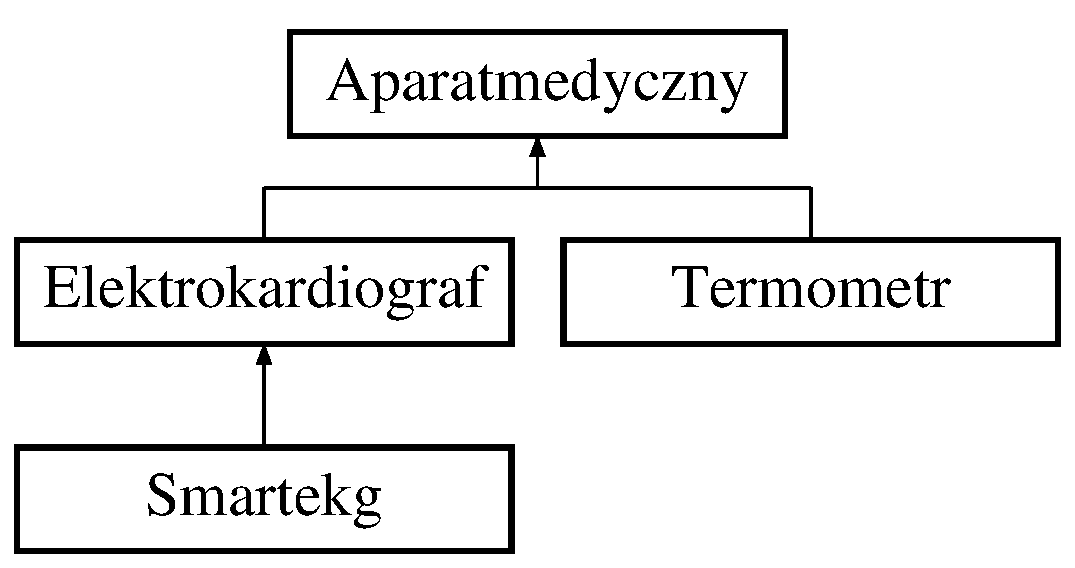
\includegraphics[height=3.000000cm]{class_aparatmedyczny}
\end{center}
\end{figure}
\subsection*{Public Member Functions}
\begin{DoxyCompactItemize}
\item 
virtual void \textbf{ wlacz} ()=0
\begin{DoxyCompactList}\small\item\em wirtualna metoda wlaczenia \end{DoxyCompactList}\item 
virtual void \textbf{ wylacz} ()=0
\begin{DoxyCompactList}\small\item\em wirtualna metoda wylaczenia \end{DoxyCompactList}\item 
virtual void \textbf{ zrobbadanie} ()=0
\begin{DoxyCompactList}\small\item\em wirtualna metoda zrobienia badania \end{DoxyCompactList}\item 
virtual void \textbf{ odczyt\+\_\+z\+\_\+pliku} (string)=0
\begin{DoxyCompactList}\small\item\em wirtualny odczyt z pliku \end{DoxyCompactList}\item 
virtual void \textbf{ zapisz\+\_\+do\+\_\+pliku} (string, int)=0
\begin{DoxyCompactList}\small\item\em wirtualny zapis do pliku \end{DoxyCompactList}\end{DoxyCompactItemize}
\subsection*{Protected Attributes}
\begin{DoxyCompactItemize}
\item 
int \textbf{ cena}
\begin{DoxyCompactList}\small\item\em $>$cena urzadzenia \end{DoxyCompactList}\item 
double \textbf{ waga}
\begin{DoxyCompactList}\small\item\em $>$waga urzadzenia \end{DoxyCompactList}\item 
double \textbf{ dlugosc}
\begin{DoxyCompactList}\small\item\em $>$dlugosc urz�dzenia \end{DoxyCompactList}\item 
double \textbf{ szerokosc}
\begin{DoxyCompactList}\small\item\em $>$szerokosc urzadzenia \end{DoxyCompactList}\end{DoxyCompactItemize}


\subsection{Detailed Description}
klasas wirtualna 

\subsection{Member Function Documentation}
\mbox{\label{class_aparatmedyczny_a5300ce8466293b738da4f2eb5ed7b233}} 
\index{Aparatmedyczny@{Aparatmedyczny}!odczyt\+\_\+z\+\_\+pliku@{odczyt\+\_\+z\+\_\+pliku}}
\index{odczyt\+\_\+z\+\_\+pliku@{odczyt\+\_\+z\+\_\+pliku}!Aparatmedyczny@{Aparatmedyczny}}
\subsubsection{odczyt\+\_\+z\+\_\+pliku()}
{\footnotesize\ttfamily virtual void Aparatmedyczny\+::odczyt\+\_\+z\+\_\+pliku (\begin{DoxyParamCaption}\item[{string}]{ }\end{DoxyParamCaption})\hspace{0.3cm}{\ttfamily [pure virtual]}}



wirtualny odczyt z pliku 



Implemented in \textbf{ Elektrokardiograf} \doxyref{}{p.}{class_elektrokardiograf_af934c2d3456229093c37310070638df2}, \textbf{ Termometr} \doxyref{}{p.}{class_termometr_a42a1dab82d6f7c1adba8b03b01d132d8}, and \textbf{ Smartekg} \doxyref{}{p.}{class_smartekg_a96fe1adb8c11601eefafe085ead3c3d1}.

\mbox{\label{class_aparatmedyczny_a303cd2ab42aa4a4a29bb59d685573c78}} 
\index{Aparatmedyczny@{Aparatmedyczny}!wlacz@{wlacz}}
\index{wlacz@{wlacz}!Aparatmedyczny@{Aparatmedyczny}}
\subsubsection{wlacz()}
{\footnotesize\ttfamily virtual void Aparatmedyczny\+::wlacz (\begin{DoxyParamCaption}{ }\end{DoxyParamCaption})\hspace{0.3cm}{\ttfamily [pure virtual]}}



wirtualna metoda wlaczenia 



Implemented in \textbf{ Elektrokardiograf} \doxyref{}{p.}{class_elektrokardiograf_a78b8311e31aa24ab92998e8105e72dd1}, \textbf{ Smartekg} \doxyref{}{p.}{class_smartekg_ab976b0a43ff21e254af74a29b4fc8688}, and \textbf{ Termometr} \doxyref{}{p.}{class_termometr_a25df4488ebce81d7c92d2c66ca02fb6d}.

\mbox{\label{class_aparatmedyczny_a0f6e8f2d4656bc258805e230ad4563d0}} 
\index{Aparatmedyczny@{Aparatmedyczny}!wylacz@{wylacz}}
\index{wylacz@{wylacz}!Aparatmedyczny@{Aparatmedyczny}}
\subsubsection{wylacz()}
{\footnotesize\ttfamily virtual void Aparatmedyczny\+::wylacz (\begin{DoxyParamCaption}{ }\end{DoxyParamCaption})\hspace{0.3cm}{\ttfamily [pure virtual]}}



wirtualna metoda wylaczenia 



Implemented in \textbf{ Elektrokardiograf} \doxyref{}{p.}{class_elektrokardiograf_aea0ea515c89cddbdde78a2edef5dc34b}, \textbf{ Smartekg} \doxyref{}{p.}{class_smartekg_a40cb07132a4139745bdf1cd31e2fd080}, and \textbf{ Termometr} \doxyref{}{p.}{class_termometr_ac13dc274e2f18f76ff8c1eb60f793a20}.

\mbox{\label{class_aparatmedyczny_aa81d3a1b324550cd90fba34d1096f772}} 
\index{Aparatmedyczny@{Aparatmedyczny}!zapisz\+\_\+do\+\_\+pliku@{zapisz\+\_\+do\+\_\+pliku}}
\index{zapisz\+\_\+do\+\_\+pliku@{zapisz\+\_\+do\+\_\+pliku}!Aparatmedyczny@{Aparatmedyczny}}
\subsubsection{zapisz\+\_\+do\+\_\+pliku()}
{\footnotesize\ttfamily virtual void Aparatmedyczny\+::zapisz\+\_\+do\+\_\+pliku (\begin{DoxyParamCaption}\item[{string}]{,  }\item[{int}]{ }\end{DoxyParamCaption})\hspace{0.3cm}{\ttfamily [pure virtual]}}



wirtualny zapis do pliku 



Implemented in \textbf{ Elektrokardiograf} \doxyref{}{p.}{class_elektrokardiograf_a7e9dc34e6867890ed9879bf5dcb5acfb}, \textbf{ Termometr} \doxyref{}{p.}{class_termometr_a852973a522848a9fbbd95361494525a4}, and \textbf{ Smartekg} \doxyref{}{p.}{class_smartekg_afb055dc43e7012d04e8764507860ffad}.

\mbox{\label{class_aparatmedyczny_adbdf7a6290c67862387d1cda2f0d9173}} 
\index{Aparatmedyczny@{Aparatmedyczny}!zrobbadanie@{zrobbadanie}}
\index{zrobbadanie@{zrobbadanie}!Aparatmedyczny@{Aparatmedyczny}}
\subsubsection{zrobbadanie()}
{\footnotesize\ttfamily virtual void Aparatmedyczny\+::zrobbadanie (\begin{DoxyParamCaption}{ }\end{DoxyParamCaption})\hspace{0.3cm}{\ttfamily [pure virtual]}}



wirtualna metoda zrobienia badania 



Implemented in \textbf{ Elektrokardiograf} \doxyref{}{p.}{class_elektrokardiograf_a4f43e5e6a427d074ee3a5acff7d96e14}, \textbf{ Smartekg} \doxyref{}{p.}{class_smartekg_a80a5495364b751184519215407ba8559}, and \textbf{ Termometr} \doxyref{}{p.}{class_termometr_acd74b1f25bb4af260d5f4f9d6baf4921}.



\subsection{Member Data Documentation}
\mbox{\label{class_aparatmedyczny_a17d894b00a60b2d3a8e4308f21570dd4}} 
\index{Aparatmedyczny@{Aparatmedyczny}!cena@{cena}}
\index{cena@{cena}!Aparatmedyczny@{Aparatmedyczny}}
\subsubsection{cena}
{\footnotesize\ttfamily int Aparatmedyczny\+::cena\hspace{0.3cm}{\ttfamily [protected]}}



$>$cena urzadzenia 

\mbox{\label{class_aparatmedyczny_a7b0688e529fb62f374a8f4bd6353cc4b}} 
\index{Aparatmedyczny@{Aparatmedyczny}!dlugosc@{dlugosc}}
\index{dlugosc@{dlugosc}!Aparatmedyczny@{Aparatmedyczny}}
\subsubsection{dlugosc}
{\footnotesize\ttfamily double Aparatmedyczny\+::dlugosc\hspace{0.3cm}{\ttfamily [protected]}}



$>$dlugosc urz�dzenia 

\mbox{\label{class_aparatmedyczny_af01e0aad8e103a60b2d46dac59d22e0a}} 
\index{Aparatmedyczny@{Aparatmedyczny}!szerokosc@{szerokosc}}
\index{szerokosc@{szerokosc}!Aparatmedyczny@{Aparatmedyczny}}
\subsubsection{szerokosc}
{\footnotesize\ttfamily double Aparatmedyczny\+::szerokosc\hspace{0.3cm}{\ttfamily [protected]}}



$>$szerokosc urzadzenia 

\mbox{\label{class_aparatmedyczny_a978a831d37de4f055cfe83b1b1b5fb52}} 
\index{Aparatmedyczny@{Aparatmedyczny}!waga@{waga}}
\index{waga@{waga}!Aparatmedyczny@{Aparatmedyczny}}
\subsubsection{waga}
{\footnotesize\ttfamily double Aparatmedyczny\+::waga\hspace{0.3cm}{\ttfamily [protected]}}



$>$waga urzadzenia 



The documentation for this class was generated from the following file\+:\begin{DoxyCompactItemize}
\item 
\textbf{ aparatmedyczny.\+h}\end{DoxyCompactItemize}

\section{Bateria Class Reference}
\label{class_bateria}\index{Bateria@{Bateria}}


\doxyref{Bateria}{p.}{class_bateria} podobiekt E\+KG.  




{\ttfamily \#include $<$bateria.\+h$>$}

\subsection*{Public Member Functions}
\begin{DoxyCompactItemize}
\item 
\textbf{ Bateria} ()
\begin{DoxyCompactList}\small\item\em konstruktor domyslny \end{DoxyCompactList}\item 
void \textbf{ zdefiniuj\+\_\+baterie} (int, int, double, string)
\begin{DoxyCompactList}\small\item\em nadanie atrybutow obiektowi \end{DoxyCompactList}\item 
\textbf{ $\sim$\+Bateria} ()
\begin{DoxyCompactList}\small\item\em destruktor \doxyref{Bateria}{p.}{class_bateria} \end{DoxyCompactList}\item 
void \textbf{ odczyt\+\_\+z\+\_\+pliku} (string)
\begin{DoxyCompactList}\small\item\em czytanie z pliku \end{DoxyCompactList}\item 
void \textbf{ zapisz\+\_\+do\+\_\+pliku} (string, int)
\begin{DoxyCompactList}\small\item\em zapisywanie do pliku \end{DoxyCompactList}\item 
void \textbf{ operator$<$$<$} (string s)
\begin{DoxyCompactList}\small\item\em operatory do zapisu w pliku przyjmujace jego nazwe \end{DoxyCompactList}\item 
void \textbf{ operator$>$$>$} (string s)
\begin{DoxyCompactList}\small\item\em operatory do odczytu z pliku przyjmujace jego nazwe \end{DoxyCompactList}\end{DoxyCompactItemize}
\subsection*{Friends}
\begin{DoxyCompactItemize}
\item 
ostream \& \textbf{ operator$<$$<$} (ostream \&wyjscie, const \textbf{ Bateria} \&s)
\begin{DoxyCompactList}\small\item\em zaprzyjazniona funkcja do wypisania obiektu za pomoca cout \end{DoxyCompactList}\end{DoxyCompactItemize}


\subsection{Detailed Description}
\doxyref{Bateria}{p.}{class_bateria} podobiekt E\+KG. 

\subsection{Constructor \& Destructor Documentation}
\mbox{\label{class_bateria_ad63fe61cc7af28c0bceea78f21097d6a}} 
\index{Bateria@{Bateria}!Bateria@{Bateria}}
\index{Bateria@{Bateria}!Bateria@{Bateria}}
\subsubsection{Bateria()}
{\footnotesize\ttfamily Bateria\+::\+Bateria (\begin{DoxyParamCaption}{ }\end{DoxyParamCaption})}



konstruktor domyslny 

\mbox{\label{class_bateria_ad3445064f0e261a342de2c1684ee3106}} 
\index{Bateria@{Bateria}!````~Bateria@{$\sim$\+Bateria}}
\index{````~Bateria@{$\sim$\+Bateria}!Bateria@{Bateria}}
\subsubsection{$\sim$\+Bateria()}
{\footnotesize\ttfamily Bateria\+::$\sim$\+Bateria (\begin{DoxyParamCaption}{ }\end{DoxyParamCaption})}



destruktor \doxyref{Bateria}{p.}{class_bateria} 



\subsection{Member Function Documentation}
\mbox{\label{class_bateria_ab07ed9d5733e40dbd567bddc076ad55a}} 
\index{Bateria@{Bateria}!odczyt\+\_\+z\+\_\+pliku@{odczyt\+\_\+z\+\_\+pliku}}
\index{odczyt\+\_\+z\+\_\+pliku@{odczyt\+\_\+z\+\_\+pliku}!Bateria@{Bateria}}
\subsubsection{odczyt\+\_\+z\+\_\+pliku()}
{\footnotesize\ttfamily void Bateria\+::odczyt\+\_\+z\+\_\+pliku (\begin{DoxyParamCaption}\item[{string}]{s }\end{DoxyParamCaption})}



czytanie z pliku 


\begin{DoxyParams}{Parameters}
{\em string} & -\/ nazwa pliku \\
\hline
\end{DoxyParams}
\mbox{\label{class_bateria_affca3230d7eb0cb04e206962f40ef7e6}} 
\index{Bateria@{Bateria}!operator$<$$<$@{operator$<$$<$}}
\index{operator$<$$<$@{operator$<$$<$}!Bateria@{Bateria}}
\subsubsection{operator$<$$<$()}
{\footnotesize\ttfamily void Bateria\+::operator$<$$<$ (\begin{DoxyParamCaption}\item[{string}]{s }\end{DoxyParamCaption})}



operatory do zapisu w pliku przyjmujace jego nazwe 

\mbox{\label{class_bateria_a6a5856b87436f0463bf65a4119482dd7}} 
\index{Bateria@{Bateria}!operator$>$$>$@{operator$>$$>$}}
\index{operator$>$$>$@{operator$>$$>$}!Bateria@{Bateria}}
\subsubsection{operator$>$$>$()}
{\footnotesize\ttfamily void Bateria\+::operator$>$$>$ (\begin{DoxyParamCaption}\item[{string}]{s }\end{DoxyParamCaption})}



operatory do odczytu z pliku przyjmujace jego nazwe 

\mbox{\label{class_bateria_a600e9c21a2605e2b493b8589c21f0467}} 
\index{Bateria@{Bateria}!zapisz\+\_\+do\+\_\+pliku@{zapisz\+\_\+do\+\_\+pliku}}
\index{zapisz\+\_\+do\+\_\+pliku@{zapisz\+\_\+do\+\_\+pliku}!Bateria@{Bateria}}
\subsubsection{zapisz\+\_\+do\+\_\+pliku()}
{\footnotesize\ttfamily void Bateria\+::zapisz\+\_\+do\+\_\+pliku (\begin{DoxyParamCaption}\item[{string}]{s,  }\item[{int}]{zapis }\end{DoxyParamCaption})}



zapisywanie do pliku 


\begin{DoxyParams}{Parameters}
{\em string} & -\/ nazwa pliku \\
\hline
{\em int} & -\/ decyduje o dopisaniu do pliku lub nadpisaniu \\
\hline
\end{DoxyParams}
\mbox{\label{class_bateria_ae61765808c0210cec772272f3d1d84d9}} 
\index{Bateria@{Bateria}!zdefiniuj\+\_\+baterie@{zdefiniuj\+\_\+baterie}}
\index{zdefiniuj\+\_\+baterie@{zdefiniuj\+\_\+baterie}!Bateria@{Bateria}}
\subsubsection{zdefiniuj\+\_\+baterie()}
{\footnotesize\ttfamily void Bateria\+::zdefiniuj\+\_\+baterie (\begin{DoxyParamCaption}\item[{int}]{p,  }\item[{int}]{cen,  }\item[{double}]{nap,  }\item[{string}]{pro }\end{DoxyParamCaption})}



nadanie atrybutow obiektowi 

Parametry to kolejno atrybuty obiektu tej klasy 

\subsection{Friends And Related Function Documentation}
\mbox{\label{class_bateria_a47035e47d5dc1f14ae25b6033bf175dc}} 
\index{Bateria@{Bateria}!operator$<$$<$@{operator$<$$<$}}
\index{operator$<$$<$@{operator$<$$<$}!Bateria@{Bateria}}
\subsubsection{operator$<$$<$}
{\footnotesize\ttfamily ostream\& operator$<$$<$ (\begin{DoxyParamCaption}\item[{ostream \&}]{wyjscie,  }\item[{const \textbf{ Bateria} \&}]{s }\end{DoxyParamCaption})\hspace{0.3cm}{\ttfamily [friend]}}



zaprzyjazniona funkcja do wypisania obiektu za pomoca cout 



The documentation for this class was generated from the following files\+:\begin{DoxyCompactItemize}
\item 
\textbf{ bateria.\+h}\item 
\textbf{ bateria.\+cpp}\end{DoxyCompactItemize}

\section{Drukarka Class Reference}
\label{class_drukarka}\index{Drukarka@{Drukarka}}


Podobiekt Elektrokardiografu.  




{\ttfamily \#include $<$drukarka.\+h$>$}

\subsection*{Public Member Functions}
\begin{DoxyCompactItemize}
\item 
\textbf{ Drukarka} ()
\begin{DoxyCompactList}\small\item\em kosntruktor domy��ny \end{DoxyCompactList}\item 
void \textbf{ ustaw\+\_\+drukarke} (int, int, int, double, string, int)
\begin{DoxyCompactList}\small\item\em ustawianie parametrow drukarki odpowiednio w kolejnosci \end{DoxyCompactList}\item 
void \textbf{ dodaj\+\_\+kartke} (string kolor)
\begin{DoxyCompactList}\small\item\em funkcja dodajaca kartke do kolejki \end{DoxyCompactList}\item 
void \textbf{ wydrukuj\+\_\+kartke} ()
\begin{DoxyCompactList}\small\item\em funkcja drukujaca kartke \end{DoxyCompactList}\item 
bool \textbf{ czypusta} ()
\begin{DoxyCompactList}\small\item\em funkcja sprawdzajaca czy jest jakas kartka /return zwraca 1 jesli brak kartek, 0 -\/ jesli jakies sa \end{DoxyCompactList}\item 
\textbf{ $\sim$\+Drukarka} ()
\begin{DoxyCompactList}\small\item\em destruktor \end{DoxyCompactList}\item 
void \textbf{ odczyt\+\_\+z\+\_\+pliku} (string)
\begin{DoxyCompactList}\small\item\em czytanie z pliku \end{DoxyCompactList}\item 
void \textbf{ zapisz\+\_\+do\+\_\+pliku} (string, int)
\begin{DoxyCompactList}\small\item\em zapisywanie do pliku \end{DoxyCompactList}\item 
void \textbf{ operator$<$$<$} (string s)
\begin{DoxyCompactList}\small\item\em operatory do zapisu w pliku przyjmujace jego nazwe \end{DoxyCompactList}\item 
void \textbf{ operator$>$$>$} (string s)
\begin{DoxyCompactList}\small\item\em operatory do odczytu z pliku przyjmujace jego nazwe \end{DoxyCompactList}\end{DoxyCompactItemize}


\subsection{Detailed Description}
Podobiekt Elektrokardiografu. 

\subsection{Constructor \& Destructor Documentation}
\mbox{\label{class_drukarka_aed4b71f0d650809ea61382a8db8bb41d}} 
\index{Drukarka@{Drukarka}!Drukarka@{Drukarka}}
\index{Drukarka@{Drukarka}!Drukarka@{Drukarka}}
\subsubsection{Drukarka()}
{\footnotesize\ttfamily Drukarka\+::\+Drukarka (\begin{DoxyParamCaption}{ }\end{DoxyParamCaption})}



kosntruktor domy��ny 

\mbox{\label{class_drukarka_a056e3d77c9c294a0870aef831985bd4d}} 
\index{Drukarka@{Drukarka}!````~Drukarka@{$\sim$\+Drukarka}}
\index{````~Drukarka@{$\sim$\+Drukarka}!Drukarka@{Drukarka}}
\subsubsection{$\sim$\+Drukarka()}
{\footnotesize\ttfamily Drukarka\+::$\sim$\+Drukarka (\begin{DoxyParamCaption}{ }\end{DoxyParamCaption})}



destruktor 



\subsection{Member Function Documentation}
\mbox{\label{class_drukarka_a1411bdffc307bda4156ff48f64db2cc5}} 
\index{Drukarka@{Drukarka}!czypusta@{czypusta}}
\index{czypusta@{czypusta}!Drukarka@{Drukarka}}
\subsubsection{czypusta()}
{\footnotesize\ttfamily bool Drukarka\+::czypusta (\begin{DoxyParamCaption}{ }\end{DoxyParamCaption})\hspace{0.3cm}{\ttfamily [inline]}}



funkcja sprawdzajaca czy jest jakas kartka /return zwraca 1 jesli brak kartek, 0 -\/ jesli jakies sa 

\mbox{\label{class_drukarka_ae30bf8712f26659417b3b06a7b8218cc}} 
\index{Drukarka@{Drukarka}!dodaj\+\_\+kartke@{dodaj\+\_\+kartke}}
\index{dodaj\+\_\+kartke@{dodaj\+\_\+kartke}!Drukarka@{Drukarka}}
\subsubsection{dodaj\+\_\+kartke()}
{\footnotesize\ttfamily void Drukarka\+::dodaj\+\_\+kartke (\begin{DoxyParamCaption}\item[{string}]{kolor }\end{DoxyParamCaption})}



funkcja dodajaca kartke do kolejki 

\mbox{\label{class_drukarka_a48627cf4f84fd13f833cebb99d5ce988}} 
\index{Drukarka@{Drukarka}!odczyt\+\_\+z\+\_\+pliku@{odczyt\+\_\+z\+\_\+pliku}}
\index{odczyt\+\_\+z\+\_\+pliku@{odczyt\+\_\+z\+\_\+pliku}!Drukarka@{Drukarka}}
\subsubsection{odczyt\+\_\+z\+\_\+pliku()}
{\footnotesize\ttfamily void Drukarka\+::odczyt\+\_\+z\+\_\+pliku (\begin{DoxyParamCaption}\item[{string}]{s }\end{DoxyParamCaption})}



czytanie z pliku 


\begin{DoxyParams}{Parameters}
{\em string} & -\/ nazwa pliku \\
\hline
\end{DoxyParams}
\mbox{\label{class_drukarka_a27bd0cbeea27ff58686601b30f75ab91}} 
\index{Drukarka@{Drukarka}!operator$<$$<$@{operator$<$$<$}}
\index{operator$<$$<$@{operator$<$$<$}!Drukarka@{Drukarka}}
\subsubsection{operator$<$$<$()}
{\footnotesize\ttfamily void Drukarka\+::operator$<$$<$ (\begin{DoxyParamCaption}\item[{string}]{s }\end{DoxyParamCaption})}



operatory do zapisu w pliku przyjmujace jego nazwe 

\mbox{\label{class_drukarka_a2371a5f120008f8034b8e847f901d4a3}} 
\index{Drukarka@{Drukarka}!operator$>$$>$@{operator$>$$>$}}
\index{operator$>$$>$@{operator$>$$>$}!Drukarka@{Drukarka}}
\subsubsection{operator$>$$>$()}
{\footnotesize\ttfamily void Drukarka\+::operator$>$$>$ (\begin{DoxyParamCaption}\item[{string}]{s }\end{DoxyParamCaption})}



operatory do odczytu z pliku przyjmujace jego nazwe 

\mbox{\label{class_drukarka_aa3d728ca6084654f34811c74c7393411}} 
\index{Drukarka@{Drukarka}!ustaw\+\_\+drukarke@{ustaw\+\_\+drukarke}}
\index{ustaw\+\_\+drukarke@{ustaw\+\_\+drukarke}!Drukarka@{Drukarka}}
\subsubsection{ustaw\+\_\+drukarke()}
{\footnotesize\ttfamily void Drukarka\+::ustaw\+\_\+drukarke (\begin{DoxyParamCaption}\item[{int}]{a,  }\item[{int}]{b,  }\item[{int}]{c,  }\item[{double}]{d,  }\item[{string}]{e,  }\item[{int}]{f }\end{DoxyParamCaption})}



ustawianie parametrow drukarki odpowiednio w kolejnosci 

\mbox{\label{class_drukarka_aa0c1eae2aaff10fca59b3d20f7449c16}} 
\index{Drukarka@{Drukarka}!wydrukuj\+\_\+kartke@{wydrukuj\+\_\+kartke}}
\index{wydrukuj\+\_\+kartke@{wydrukuj\+\_\+kartke}!Drukarka@{Drukarka}}
\subsubsection{wydrukuj\+\_\+kartke()}
{\footnotesize\ttfamily void Drukarka\+::wydrukuj\+\_\+kartke (\begin{DoxyParamCaption}{ }\end{DoxyParamCaption})}



funkcja drukujaca kartke 

\mbox{\label{class_drukarka_aba9bba44a8c07a47760840268bb96b05}} 
\index{Drukarka@{Drukarka}!zapisz\+\_\+do\+\_\+pliku@{zapisz\+\_\+do\+\_\+pliku}}
\index{zapisz\+\_\+do\+\_\+pliku@{zapisz\+\_\+do\+\_\+pliku}!Drukarka@{Drukarka}}
\subsubsection{zapisz\+\_\+do\+\_\+pliku()}
{\footnotesize\ttfamily void Drukarka\+::zapisz\+\_\+do\+\_\+pliku (\begin{DoxyParamCaption}\item[{string}]{s,  }\item[{int}]{zapis }\end{DoxyParamCaption})}



zapisywanie do pliku 


\begin{DoxyParams}{Parameters}
{\em string} & -\/ nazwa pliku \\
\hline
{\em int} & -\/ decyduje o dopisaniu do pliku lub nadpisaniu \\
\hline
\end{DoxyParams}


The documentation for this class was generated from the following files\+:\begin{DoxyCompactItemize}
\item 
\textbf{ drukarka.\+h}\item 
\textbf{ drukarka.\+cpp}\end{DoxyCompactItemize}

\section{Elektrokardiograf Class Reference}
\label{class_elektrokardiograf}\index{Elektrokardiograf@{Elektrokardiograf}}


klasa \doxyref{Elektrokardiograf}{p.}{class_elektrokardiograf} obiekt glowny dziedziczaca po \doxyref{Aparatmedyczny}{p.}{class_aparatmedyczny}  




{\ttfamily \#include $<$elektrokardiograf.\+h$>$}

Inheritance diagram for Elektrokardiograf\+:\begin{figure}[H]
\begin{center}
\leavevmode
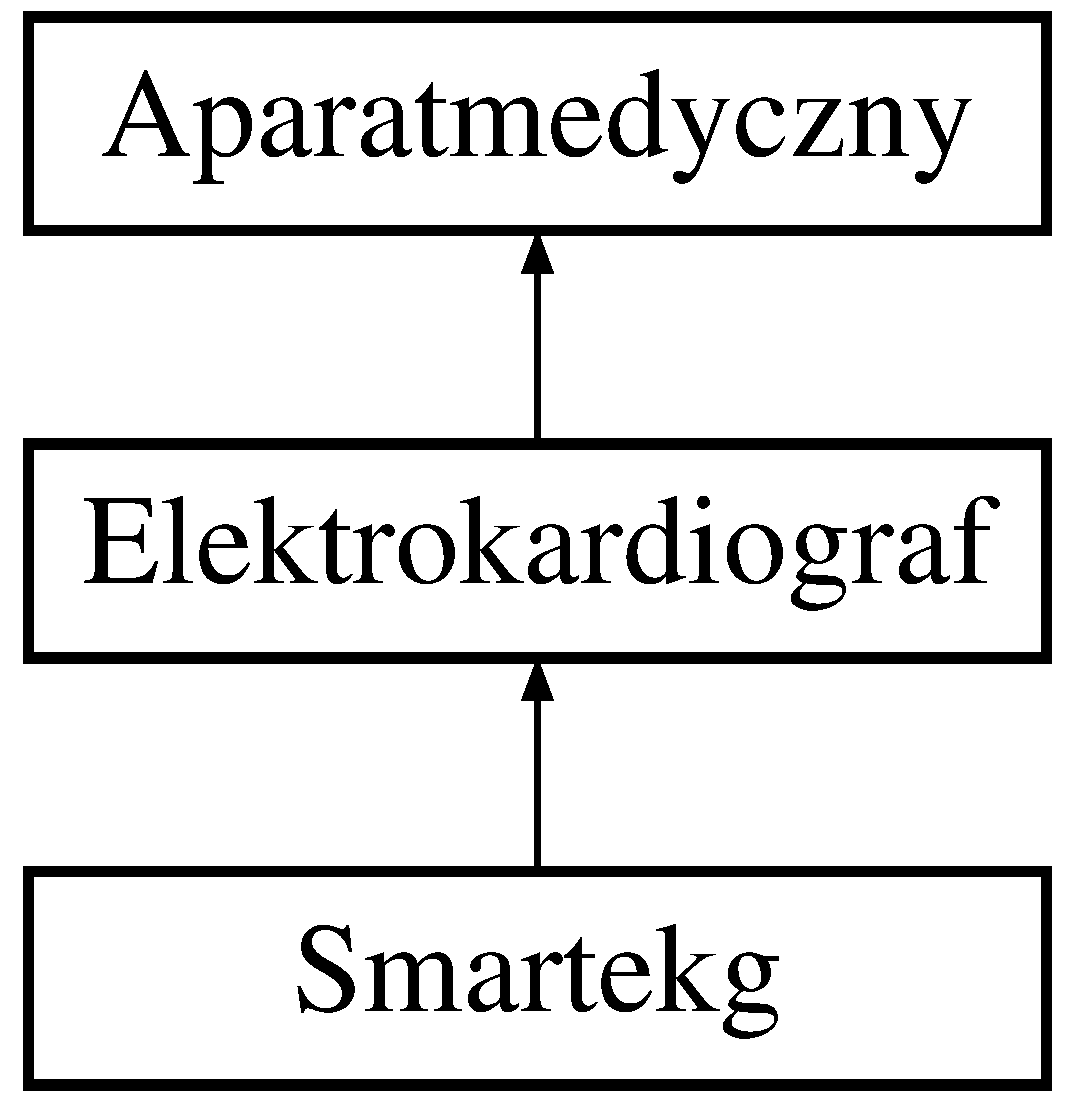
\includegraphics[height=3.000000cm]{class_elektrokardiograf}
\end{center}
\end{figure}
\subsection*{Public Member Functions}
\begin{DoxyCompactItemize}
\item 
\textbf{ Elektrokardiograf} ()
\begin{DoxyCompactList}\small\item\em konstruktor domyslny \end{DoxyCompactList}\item 
\textbf{ Elektrokardiograf} (const \textbf{ Elektrokardiograf} \&obs)
\begin{DoxyCompactList}\small\item\em konstruktor kopiujacy \end{DoxyCompactList}\item 
\textbf{ Elektrokardiograf} (int a, double c, double d, double e, double f, string nazwa, string model1)
\begin{DoxyCompactList}\small\item\em konstruktor z parametrami \end{DoxyCompactList}\item 
void \textbf{ wlacz} ()
\begin{DoxyCompactList}\small\item\em wirtualna metoda wlaczenia przyrzadu \end{DoxyCompactList}\item 
void \textbf{ wylacz} ()
\begin{DoxyCompactList}\small\item\em wirtualna metoda wylaczenia przyrzadu \end{DoxyCompactList}\item 
void \textbf{ zrobbadanie} ()
\begin{DoxyCompactList}\small\item\em metoda \char`\"{}symulujaca\char`\"{} badania \end{DoxyCompactList}\item 
void \textbf{ nadaj\+\_\+\+Wartosci} (int a, double c, double d, double e, double f, string nazwa, string model1)
\begin{DoxyCompactList}\small\item\em funkcja nadajaca wartosci \end{DoxyCompactList}\item 
double \textbf{ zwroc\+\_\+\+Powierzchnie} ()
\begin{DoxyCompactList}\small\item\em funkcja zwraca powierzchnie /return zwraca wynik w double \end{DoxyCompactList}\item 
double \textbf{ zwroc\+\_\+\+Wage} ()
\begin{DoxyCompactList}\small\item\em funkcja zwraca wage /return zwraca wynik w double \end{DoxyCompactList}\item 
\textbf{ Wyswietlacz} $\ast$ \textbf{ zwroc\+\_\+\+Wyswietlacz} ()
\begin{DoxyCompactList}\small\item\em zwraca wyswietlacz podobiekt Elektrokardiografu /return zwraca wskaznik na drukarke \end{DoxyCompactList}\item 
\textbf{ Drukarka} $\ast$ \textbf{ zwroc\+\_\+\+Drukarke} ()
\begin{DoxyCompactList}\small\item\em zwraca drukarke podobiekt Elektrokardiografu /return zwraca wskaznik na drukarke \end{DoxyCompactList}\item 
void \textbf{ wloz\+\_\+\+Baterie} (int sztuki)
\begin{DoxyCompactList}\small\item\em wklada baterie do urzadzenia \end{DoxyCompactList}\item 
\textbf{ $\sim$\+Elektrokardiograf} ()
\begin{DoxyCompactList}\small\item\em destruktor Elektrokardiorafu \end{DoxyCompactList}\item 
bool \textbf{ operator==} (const \textbf{ Elektrokardiograf} \&s)
\begin{DoxyCompactList}\small\item\em operator porownania \end{DoxyCompactList}\item 
void \textbf{ operator=} (const \textbf{ Elektrokardiograf} \&s)
\begin{DoxyCompactList}\small\item\em operator pzypisania \end{DoxyCompactList}\item 
\textbf{ Bateria} \& \textbf{ operator[$\,$]} (int a)
\begin{DoxyCompactList}\small\item\em operator indeksowania /return zwraca wskaznik na baterie \end{DoxyCompactList}\item 
\textbf{ operator int} () const
\begin{DoxyCompactList}\small\item\em operator konwersji \end{DoxyCompactList}\item 
\textbf{ Elektrokardiograf} $\ast$ \textbf{ operator++} (int n)
\begin{DoxyCompactList}\small\item\em operator inkrementacji /return zwraca ten sam obiekt z powiekszonym czasem \end{DoxyCompactList}\item 
void \textbf{ operator$<$$<$} (string s)
\begin{DoxyCompactList}\small\item\em operatory do zapisu w pliku przyjmujace jego nazwe \end{DoxyCompactList}\item 
void \textbf{ operator$>$$>$} (string s)
\begin{DoxyCompactList}\small\item\em operatory do odczytu z pliku przyjmujace jego nazwe \end{DoxyCompactList}\item 
void \textbf{ odczyt\+\_\+z\+\_\+pliku} (string)
\begin{DoxyCompactList}\small\item\em czytanie z pliku \end{DoxyCompactList}\item 
void \textbf{ zapisz\+\_\+do\+\_\+pliku} (string, int)
\begin{DoxyCompactList}\small\item\em zapisywanie do pliku \end{DoxyCompactList}\end{DoxyCompactItemize}
\subsection*{Static Public Member Functions}
\begin{DoxyCompactItemize}
\item 
static int \textbf{ zwroc\+\_\+\+Liczbe\+\_\+\+Obiektow} ()
\begin{DoxyCompactList}\small\item\em statyczna skladowa /return Zwraca ilo�� obiektow \end{DoxyCompactList}\end{DoxyCompactItemize}
\subsection*{Protected Attributes}
\begin{DoxyCompactItemize}
\item 
double \textbf{ czas\+\_\+pomiaru}
\begin{DoxyCompactList}\small\item\em $>$czas pomiaru \end{DoxyCompactList}\item 
string \textbf{ producent}
\begin{DoxyCompactList}\small\item\em $>$producent \end{DoxyCompactList}\item 
string \textbf{ model}
\begin{DoxyCompactList}\small\item\em $>$model \end{DoxyCompactList}\item 
vector$<$ \textbf{ Bateria} $\ast$ $>$ \textbf{ bateria}
\begin{DoxyCompactList}\small\item\em $>$podobiekt bateria \end{DoxyCompactList}\item 
\textbf{ Wyswietlacz} \textbf{ wyswietlacz}
\begin{DoxyCompactList}\small\item\em $>$podobiekt wyswietlacz \end{DoxyCompactList}\item 
\textbf{ Drukarka} \textbf{ drukarka}
\begin{DoxyCompactList}\small\item\em $>$podobiekt drukarka \end{DoxyCompactList}\item 
bool \textbf{ dziala}
\begin{DoxyCompactList}\small\item\em $>$czy ekg wlaczone \end{DoxyCompactList}\end{DoxyCompactItemize}
\subsection*{Friends}
\begin{DoxyCompactItemize}
\item 
ostream \& \textbf{ operator$<$$<$} (ostream \&wyjscie, const \textbf{ Elektrokardiograf} \&s)
\begin{DoxyCompactList}\small\item\em zaprzyjazniona funkcja do wypisania obiektu za pomoca cout \end{DoxyCompactList}\end{DoxyCompactItemize}


\subsection{Detailed Description}
klasa \doxyref{Elektrokardiograf}{p.}{class_elektrokardiograf} obiekt glowny dziedziczaca po \doxyref{Aparatmedyczny}{p.}{class_aparatmedyczny} 

\subsection{Constructor \& Destructor Documentation}
\mbox{\label{class_elektrokardiograf_a30f0bcd7ee08a19b400bd600543379b6}} 
\index{Elektrokardiograf@{Elektrokardiograf}!Elektrokardiograf@{Elektrokardiograf}}
\index{Elektrokardiograf@{Elektrokardiograf}!Elektrokardiograf@{Elektrokardiograf}}
\subsubsection{Elektrokardiograf()\hspace{0.1cm}{\footnotesize\ttfamily [1/3]}}
{\footnotesize\ttfamily Elektrokardiograf\+::\+Elektrokardiograf (\begin{DoxyParamCaption}{ }\end{DoxyParamCaption})}



konstruktor domyslny 

\mbox{\label{class_elektrokardiograf_a1c0dbfd5445007f58bd855f166588ceb}} 
\index{Elektrokardiograf@{Elektrokardiograf}!Elektrokardiograf@{Elektrokardiograf}}
\index{Elektrokardiograf@{Elektrokardiograf}!Elektrokardiograf@{Elektrokardiograf}}
\subsubsection{Elektrokardiograf()\hspace{0.1cm}{\footnotesize\ttfamily [2/3]}}
{\footnotesize\ttfamily Elektrokardiograf\+::\+Elektrokardiograf (\begin{DoxyParamCaption}\item[{const \textbf{ Elektrokardiograf} \&}]{obs }\end{DoxyParamCaption})}



konstruktor kopiujacy 

\mbox{\label{class_elektrokardiograf_a6a62071e7e101afa1263bcee46987a10}} 
\index{Elektrokardiograf@{Elektrokardiograf}!Elektrokardiograf@{Elektrokardiograf}}
\index{Elektrokardiograf@{Elektrokardiograf}!Elektrokardiograf@{Elektrokardiograf}}
\subsubsection{Elektrokardiograf()\hspace{0.1cm}{\footnotesize\ttfamily [3/3]}}
{\footnotesize\ttfamily Elektrokardiograf\+::\+Elektrokardiograf (\begin{DoxyParamCaption}\item[{int}]{a,  }\item[{double}]{c,  }\item[{double}]{d,  }\item[{double}]{e,  }\item[{double}]{f,  }\item[{string}]{nazwa,  }\item[{string}]{model1 }\end{DoxyParamCaption})}



konstruktor z parametrami 

/param a to cena /param c to waga /param d to dlugosc /param e to szerokosc /param f to czas mierzenia /param nazwa to producent /param model1 to model \mbox{\label{class_elektrokardiograf_ace0c008d547bcbe4bff945bea6a9336b}} 
\index{Elektrokardiograf@{Elektrokardiograf}!````~Elektrokardiograf@{$\sim$\+Elektrokardiograf}}
\index{````~Elektrokardiograf@{$\sim$\+Elektrokardiograf}!Elektrokardiograf@{Elektrokardiograf}}
\subsubsection{$\sim$\+Elektrokardiograf()}
{\footnotesize\ttfamily Elektrokardiograf\+::$\sim$\+Elektrokardiograf (\begin{DoxyParamCaption}{ }\end{DoxyParamCaption})}



destruktor Elektrokardiorafu 



\subsection{Member Function Documentation}
\mbox{\label{class_elektrokardiograf_a63ac999eaec3be1f13410f64668ee4f1}} 
\index{Elektrokardiograf@{Elektrokardiograf}!nadaj\+\_\+\+Wartosci@{nadaj\+\_\+\+Wartosci}}
\index{nadaj\+\_\+\+Wartosci@{nadaj\+\_\+\+Wartosci}!Elektrokardiograf@{Elektrokardiograf}}
\subsubsection{nadaj\+\_\+\+Wartosci()}
{\footnotesize\ttfamily void Elektrokardiograf\+::nadaj\+\_\+\+Wartosci (\begin{DoxyParamCaption}\item[{int}]{a,  }\item[{double}]{c,  }\item[{double}]{d,  }\item[{double}]{e,  }\item[{double}]{f,  }\item[{string}]{nazwa,  }\item[{string}]{model1 }\end{DoxyParamCaption})}



funkcja nadajaca wartosci 

/param a to cena /param c to waga /param d to dlugosc /param e to szerokosc /param f to czas mierzenia /param nazwa to producent /param model1 to model \mbox{\label{class_elektrokardiograf_af934c2d3456229093c37310070638df2}} 
\index{Elektrokardiograf@{Elektrokardiograf}!odczyt\+\_\+z\+\_\+pliku@{odczyt\+\_\+z\+\_\+pliku}}
\index{odczyt\+\_\+z\+\_\+pliku@{odczyt\+\_\+z\+\_\+pliku}!Elektrokardiograf@{Elektrokardiograf}}
\subsubsection{odczyt\+\_\+z\+\_\+pliku()}
{\footnotesize\ttfamily void Elektrokardiograf\+::odczyt\+\_\+z\+\_\+pliku (\begin{DoxyParamCaption}\item[{string}]{s }\end{DoxyParamCaption})\hspace{0.3cm}{\ttfamily [virtual]}}



czytanie z pliku 


\begin{DoxyParams}{Parameters}
{\em string} & -\/ nazwa pliku \\
\hline
\end{DoxyParams}


Implements \textbf{ Aparatmedyczny} \doxyref{}{p.}{class_aparatmedyczny_a5300ce8466293b738da4f2eb5ed7b233}.



Reimplemented in \textbf{ Smartekg} \doxyref{}{p.}{class_smartekg_a96fe1adb8c11601eefafe085ead3c3d1}.

\mbox{\label{class_elektrokardiograf_a5862a0ddabeb36d539b18c1a764e1910}} 
\index{Elektrokardiograf@{Elektrokardiograf}!operator int@{operator int}}
\index{operator int@{operator int}!Elektrokardiograf@{Elektrokardiograf}}
\subsubsection{operator int()}
{\footnotesize\ttfamily Elektrokardiograf\+::operator int (\begin{DoxyParamCaption}{ }\end{DoxyParamCaption}) const\hspace{0.3cm}{\ttfamily [inline]}}



operator konwersji 

\mbox{\label{class_elektrokardiograf_a96f876b75c35c3399fda3f87949bc74d}} 
\index{Elektrokardiograf@{Elektrokardiograf}!operator++@{operator++}}
\index{operator++@{operator++}!Elektrokardiograf@{Elektrokardiograf}}
\subsubsection{operator++()}
{\footnotesize\ttfamily \textbf{ Elektrokardiograf}$\ast$ Elektrokardiograf\+::operator++ (\begin{DoxyParamCaption}\item[{int}]{n }\end{DoxyParamCaption})\hspace{0.3cm}{\ttfamily [inline]}}



operator inkrementacji /return zwraca ten sam obiekt z powiekszonym czasem 

\mbox{\label{class_elektrokardiograf_af04130d876dc037e0f4fcddc623885c5}} 
\index{Elektrokardiograf@{Elektrokardiograf}!operator$<$$<$@{operator$<$$<$}}
\index{operator$<$$<$@{operator$<$$<$}!Elektrokardiograf@{Elektrokardiograf}}
\subsubsection{operator$<$$<$()}
{\footnotesize\ttfamily void Elektrokardiograf\+::operator$<$$<$ (\begin{DoxyParamCaption}\item[{string}]{s }\end{DoxyParamCaption})}



operatory do zapisu w pliku przyjmujace jego nazwe 

\mbox{\label{class_elektrokardiograf_a3a074ae206fb60425828976853692482}} 
\index{Elektrokardiograf@{Elektrokardiograf}!operator=@{operator=}}
\index{operator=@{operator=}!Elektrokardiograf@{Elektrokardiograf}}
\subsubsection{operator=()}
{\footnotesize\ttfamily void Elektrokardiograf\+::operator= (\begin{DoxyParamCaption}\item[{const \textbf{ Elektrokardiograf} \&}]{s }\end{DoxyParamCaption})}



operator pzypisania 

\mbox{\label{class_elektrokardiograf_ad9618c686dc77d6e4b5b53fc691e1f3d}} 
\index{Elektrokardiograf@{Elektrokardiograf}!operator==@{operator==}}
\index{operator==@{operator==}!Elektrokardiograf@{Elektrokardiograf}}
\subsubsection{operator==()}
{\footnotesize\ttfamily bool Elektrokardiograf\+::operator== (\begin{DoxyParamCaption}\item[{const \textbf{ Elektrokardiograf} \&}]{s }\end{DoxyParamCaption})}



operator porownania 

\mbox{\label{class_elektrokardiograf_aea353bd56981c8407a506817bd95c777}} 
\index{Elektrokardiograf@{Elektrokardiograf}!operator$>$$>$@{operator$>$$>$}}
\index{operator$>$$>$@{operator$>$$>$}!Elektrokardiograf@{Elektrokardiograf}}
\subsubsection{operator$>$$>$()}
{\footnotesize\ttfamily void Elektrokardiograf\+::operator$>$$>$ (\begin{DoxyParamCaption}\item[{string}]{s }\end{DoxyParamCaption})}



operatory do odczytu z pliku przyjmujace jego nazwe 

\mbox{\label{class_elektrokardiograf_ad73eda999999956ad1e7e68b627dfd7e}} 
\index{Elektrokardiograf@{Elektrokardiograf}!operator[]@{operator[]}}
\index{operator[]@{operator[]}!Elektrokardiograf@{Elektrokardiograf}}
\subsubsection{operator[]()}
{\footnotesize\ttfamily \textbf{ Bateria} \& Elektrokardiograf\+::operator[$\,$] (\begin{DoxyParamCaption}\item[{int}]{a }\end{DoxyParamCaption})}



operator indeksowania /return zwraca wskaznik na baterie 

\mbox{\label{class_elektrokardiograf_a78b8311e31aa24ab92998e8105e72dd1}} 
\index{Elektrokardiograf@{Elektrokardiograf}!wlacz@{wlacz}}
\index{wlacz@{wlacz}!Elektrokardiograf@{Elektrokardiograf}}
\subsubsection{wlacz()}
{\footnotesize\ttfamily void Elektrokardiograf\+::wlacz (\begin{DoxyParamCaption}{ }\end{DoxyParamCaption})\hspace{0.3cm}{\ttfamily [virtual]}}



wirtualna metoda wlaczenia przyrzadu 



Implements \textbf{ Aparatmedyczny} \doxyref{}{p.}{class_aparatmedyczny_a303cd2ab42aa4a4a29bb59d685573c78}.



Reimplemented in \textbf{ Smartekg} \doxyref{}{p.}{class_smartekg_ab976b0a43ff21e254af74a29b4fc8688}.

\mbox{\label{class_elektrokardiograf_a11a6a56b4a61b660b928549cdc6d35f8}} 
\index{Elektrokardiograf@{Elektrokardiograf}!wloz\+\_\+\+Baterie@{wloz\+\_\+\+Baterie}}
\index{wloz\+\_\+\+Baterie@{wloz\+\_\+\+Baterie}!Elektrokardiograf@{Elektrokardiograf}}
\subsubsection{wloz\+\_\+\+Baterie()}
{\footnotesize\ttfamily void Elektrokardiograf\+::wloz\+\_\+\+Baterie (\begin{DoxyParamCaption}\item[{int}]{sztuki }\end{DoxyParamCaption})}



wklada baterie do urzadzenia 

\mbox{\label{class_elektrokardiograf_aea0ea515c89cddbdde78a2edef5dc34b}} 
\index{Elektrokardiograf@{Elektrokardiograf}!wylacz@{wylacz}}
\index{wylacz@{wylacz}!Elektrokardiograf@{Elektrokardiograf}}
\subsubsection{wylacz()}
{\footnotesize\ttfamily void Elektrokardiograf\+::wylacz (\begin{DoxyParamCaption}{ }\end{DoxyParamCaption})\hspace{0.3cm}{\ttfamily [virtual]}}



wirtualna metoda wylaczenia przyrzadu 



Implements \textbf{ Aparatmedyczny} \doxyref{}{p.}{class_aparatmedyczny_a0f6e8f2d4656bc258805e230ad4563d0}.



Reimplemented in \textbf{ Smartekg} \doxyref{}{p.}{class_smartekg_a40cb07132a4139745bdf1cd31e2fd080}.

\mbox{\label{class_elektrokardiograf_a7e9dc34e6867890ed9879bf5dcb5acfb}} 
\index{Elektrokardiograf@{Elektrokardiograf}!zapisz\+\_\+do\+\_\+pliku@{zapisz\+\_\+do\+\_\+pliku}}
\index{zapisz\+\_\+do\+\_\+pliku@{zapisz\+\_\+do\+\_\+pliku}!Elektrokardiograf@{Elektrokardiograf}}
\subsubsection{zapisz\+\_\+do\+\_\+pliku()}
{\footnotesize\ttfamily void Elektrokardiograf\+::zapisz\+\_\+do\+\_\+pliku (\begin{DoxyParamCaption}\item[{string}]{s,  }\item[{int}]{zapis }\end{DoxyParamCaption})\hspace{0.3cm}{\ttfamily [virtual]}}



zapisywanie do pliku 


\begin{DoxyParams}{Parameters}
{\em string} & -\/ nazwa pliku \\
\hline
{\em int} & -\/ decyduje o dopisaniu do pliku lub nadpisaniu \\
\hline
\end{DoxyParams}


Implements \textbf{ Aparatmedyczny} \doxyref{}{p.}{class_aparatmedyczny_aa81d3a1b324550cd90fba34d1096f772}.



Reimplemented in \textbf{ Smartekg} \doxyref{}{p.}{class_smartekg_afb055dc43e7012d04e8764507860ffad}.

\mbox{\label{class_elektrokardiograf_a4f43e5e6a427d074ee3a5acff7d96e14}} 
\index{Elektrokardiograf@{Elektrokardiograf}!zrobbadanie@{zrobbadanie}}
\index{zrobbadanie@{zrobbadanie}!Elektrokardiograf@{Elektrokardiograf}}
\subsubsection{zrobbadanie()}
{\footnotesize\ttfamily void Elektrokardiograf\+::zrobbadanie (\begin{DoxyParamCaption}{ }\end{DoxyParamCaption})\hspace{0.3cm}{\ttfamily [virtual]}}



metoda \char`\"{}symulujaca\char`\"{} badania 



Implements \textbf{ Aparatmedyczny} \doxyref{}{p.}{class_aparatmedyczny_adbdf7a6290c67862387d1cda2f0d9173}.



Reimplemented in \textbf{ Smartekg} \doxyref{}{p.}{class_smartekg_a80a5495364b751184519215407ba8559}.

\mbox{\label{class_elektrokardiograf_a659d2860924ba13b2d0aff689d8e28e6}} 
\index{Elektrokardiograf@{Elektrokardiograf}!zwroc\+\_\+\+Drukarke@{zwroc\+\_\+\+Drukarke}}
\index{zwroc\+\_\+\+Drukarke@{zwroc\+\_\+\+Drukarke}!Elektrokardiograf@{Elektrokardiograf}}
\subsubsection{zwroc\+\_\+\+Drukarke()}
{\footnotesize\ttfamily \textbf{ Drukarka}$\ast$ Elektrokardiograf\+::zwroc\+\_\+\+Drukarke (\begin{DoxyParamCaption}{ }\end{DoxyParamCaption})\hspace{0.3cm}{\ttfamily [inline]}}



zwraca drukarke podobiekt Elektrokardiografu /return zwraca wskaznik na drukarke 

\mbox{\label{class_elektrokardiograf_ad9e2a8ebaf0d5204d5c8c4663069a4d6}} 
\index{Elektrokardiograf@{Elektrokardiograf}!zwroc\+\_\+\+Liczbe\+\_\+\+Obiektow@{zwroc\+\_\+\+Liczbe\+\_\+\+Obiektow}}
\index{zwroc\+\_\+\+Liczbe\+\_\+\+Obiektow@{zwroc\+\_\+\+Liczbe\+\_\+\+Obiektow}!Elektrokardiograf@{Elektrokardiograf}}
\subsubsection{zwroc\+\_\+\+Liczbe\+\_\+\+Obiektow()}
{\footnotesize\ttfamily static int Elektrokardiograf\+::zwroc\+\_\+\+Liczbe\+\_\+\+Obiektow (\begin{DoxyParamCaption}{ }\end{DoxyParamCaption})\hspace{0.3cm}{\ttfamily [inline]}, {\ttfamily [static]}}



statyczna skladowa /return Zwraca ilo�� obiektow 

\mbox{\label{class_elektrokardiograf_a6129e08563cbad6fff62658cd8cbc5b7}} 
\index{Elektrokardiograf@{Elektrokardiograf}!zwroc\+\_\+\+Powierzchnie@{zwroc\+\_\+\+Powierzchnie}}
\index{zwroc\+\_\+\+Powierzchnie@{zwroc\+\_\+\+Powierzchnie}!Elektrokardiograf@{Elektrokardiograf}}
\subsubsection{zwroc\+\_\+\+Powierzchnie()}
{\footnotesize\ttfamily double Elektrokardiograf\+::zwroc\+\_\+\+Powierzchnie (\begin{DoxyParamCaption}{ }\end{DoxyParamCaption})\hspace{0.3cm}{\ttfamily [inline]}}



funkcja zwraca powierzchnie /return zwraca wynik w double 

\mbox{\label{class_elektrokardiograf_af64e5bf8b4f5293c7063b48dcc1e191a}} 
\index{Elektrokardiograf@{Elektrokardiograf}!zwroc\+\_\+\+Wage@{zwroc\+\_\+\+Wage}}
\index{zwroc\+\_\+\+Wage@{zwroc\+\_\+\+Wage}!Elektrokardiograf@{Elektrokardiograf}}
\subsubsection{zwroc\+\_\+\+Wage()}
{\footnotesize\ttfamily double Elektrokardiograf\+::zwroc\+\_\+\+Wage (\begin{DoxyParamCaption}{ }\end{DoxyParamCaption})\hspace{0.3cm}{\ttfamily [inline]}}



funkcja zwraca wage /return zwraca wynik w double 

\mbox{\label{class_elektrokardiograf_a32cb306a39462a50e5eb27c7eb673fc4}} 
\index{Elektrokardiograf@{Elektrokardiograf}!zwroc\+\_\+\+Wyswietlacz@{zwroc\+\_\+\+Wyswietlacz}}
\index{zwroc\+\_\+\+Wyswietlacz@{zwroc\+\_\+\+Wyswietlacz}!Elektrokardiograf@{Elektrokardiograf}}
\subsubsection{zwroc\+\_\+\+Wyswietlacz()}
{\footnotesize\ttfamily \textbf{ Wyswietlacz}$\ast$ Elektrokardiograf\+::zwroc\+\_\+\+Wyswietlacz (\begin{DoxyParamCaption}{ }\end{DoxyParamCaption})\hspace{0.3cm}{\ttfamily [inline]}}



zwraca wyswietlacz podobiekt Elektrokardiografu /return zwraca wskaznik na drukarke 



\subsection{Friends And Related Function Documentation}
\mbox{\label{class_elektrokardiograf_a10836bab7baab06a7a2a5d276b1eee15}} 
\index{Elektrokardiograf@{Elektrokardiograf}!operator$<$$<$@{operator$<$$<$}}
\index{operator$<$$<$@{operator$<$$<$}!Elektrokardiograf@{Elektrokardiograf}}
\subsubsection{operator$<$$<$}
{\footnotesize\ttfamily ostream\& operator$<$$<$ (\begin{DoxyParamCaption}\item[{ostream \&}]{wyjscie,  }\item[{const \textbf{ Elektrokardiograf} \&}]{s }\end{DoxyParamCaption})\hspace{0.3cm}{\ttfamily [friend]}}



zaprzyjazniona funkcja do wypisania obiektu za pomoca cout 



\subsection{Member Data Documentation}
\mbox{\label{class_elektrokardiograf_aca6f454b6817213106933e061db14628}} 
\index{Elektrokardiograf@{Elektrokardiograf}!bateria@{bateria}}
\index{bateria@{bateria}!Elektrokardiograf@{Elektrokardiograf}}
\subsubsection{bateria}
{\footnotesize\ttfamily vector$<$\textbf{ Bateria}$\ast$$>$ Elektrokardiograf\+::bateria\hspace{0.3cm}{\ttfamily [protected]}}



$>$podobiekt bateria 

\mbox{\label{class_elektrokardiograf_a0cd94c208110b3be5cf00e8bb4ca6fa5}} 
\index{Elektrokardiograf@{Elektrokardiograf}!czas\+\_\+pomiaru@{czas\+\_\+pomiaru}}
\index{czas\+\_\+pomiaru@{czas\+\_\+pomiaru}!Elektrokardiograf@{Elektrokardiograf}}
\subsubsection{czas\+\_\+pomiaru}
{\footnotesize\ttfamily double Elektrokardiograf\+::czas\+\_\+pomiaru\hspace{0.3cm}{\ttfamily [protected]}}



$>$czas pomiaru 

\mbox{\label{class_elektrokardiograf_afba139d7468fbd9f13505fa0877cf286}} 
\index{Elektrokardiograf@{Elektrokardiograf}!drukarka@{drukarka}}
\index{drukarka@{drukarka}!Elektrokardiograf@{Elektrokardiograf}}
\subsubsection{drukarka}
{\footnotesize\ttfamily \textbf{ Drukarka} Elektrokardiograf\+::drukarka\hspace{0.3cm}{\ttfamily [protected]}}



$>$podobiekt drukarka 

\mbox{\label{class_elektrokardiograf_a96589f238ff0be38b7201fc4f82ff2f7}} 
\index{Elektrokardiograf@{Elektrokardiograf}!dziala@{dziala}}
\index{dziala@{dziala}!Elektrokardiograf@{Elektrokardiograf}}
\subsubsection{dziala}
{\footnotesize\ttfamily bool Elektrokardiograf\+::dziala\hspace{0.3cm}{\ttfamily [protected]}}



$>$czy ekg wlaczone 

\mbox{\label{class_elektrokardiograf_a43f5b38916de61b6771018d5921711e5}} 
\index{Elektrokardiograf@{Elektrokardiograf}!model@{model}}
\index{model@{model}!Elektrokardiograf@{Elektrokardiograf}}
\subsubsection{model}
{\footnotesize\ttfamily string Elektrokardiograf\+::model\hspace{0.3cm}{\ttfamily [protected]}}



$>$model 

\mbox{\label{class_elektrokardiograf_a92c3c2e00c0565ed15425c639e576a6a}} 
\index{Elektrokardiograf@{Elektrokardiograf}!producent@{producent}}
\index{producent@{producent}!Elektrokardiograf@{Elektrokardiograf}}
\subsubsection{producent}
{\footnotesize\ttfamily string Elektrokardiograf\+::producent\hspace{0.3cm}{\ttfamily [protected]}}



$>$producent 

\mbox{\label{class_elektrokardiograf_a910aaecae3b43b63a157c386dc27bcaa}} 
\index{Elektrokardiograf@{Elektrokardiograf}!wyswietlacz@{wyswietlacz}}
\index{wyswietlacz@{wyswietlacz}!Elektrokardiograf@{Elektrokardiograf}}
\subsubsection{wyswietlacz}
{\footnotesize\ttfamily \textbf{ Wyswietlacz} Elektrokardiograf\+::wyswietlacz\hspace{0.3cm}{\ttfamily [protected]}}



$>$podobiekt wyswietlacz 



The documentation for this class was generated from the following files\+:\begin{DoxyCompactItemize}
\item 
\textbf{ elektrokardiograf.\+h}\item 
\textbf{ elektrokardiograf.\+cpp}\end{DoxyCompactItemize}

\section{Smartekg Class Reference}
\label{class_smartekg}\index{Smartekg@{Smartekg}}


Klasa pochodna Elektrokardiografu.  




{\ttfamily \#include $<$smartekg.\+h$>$}

Inheritance diagram for Smartekg\+:\begin{figure}[H]
\begin{center}
\leavevmode
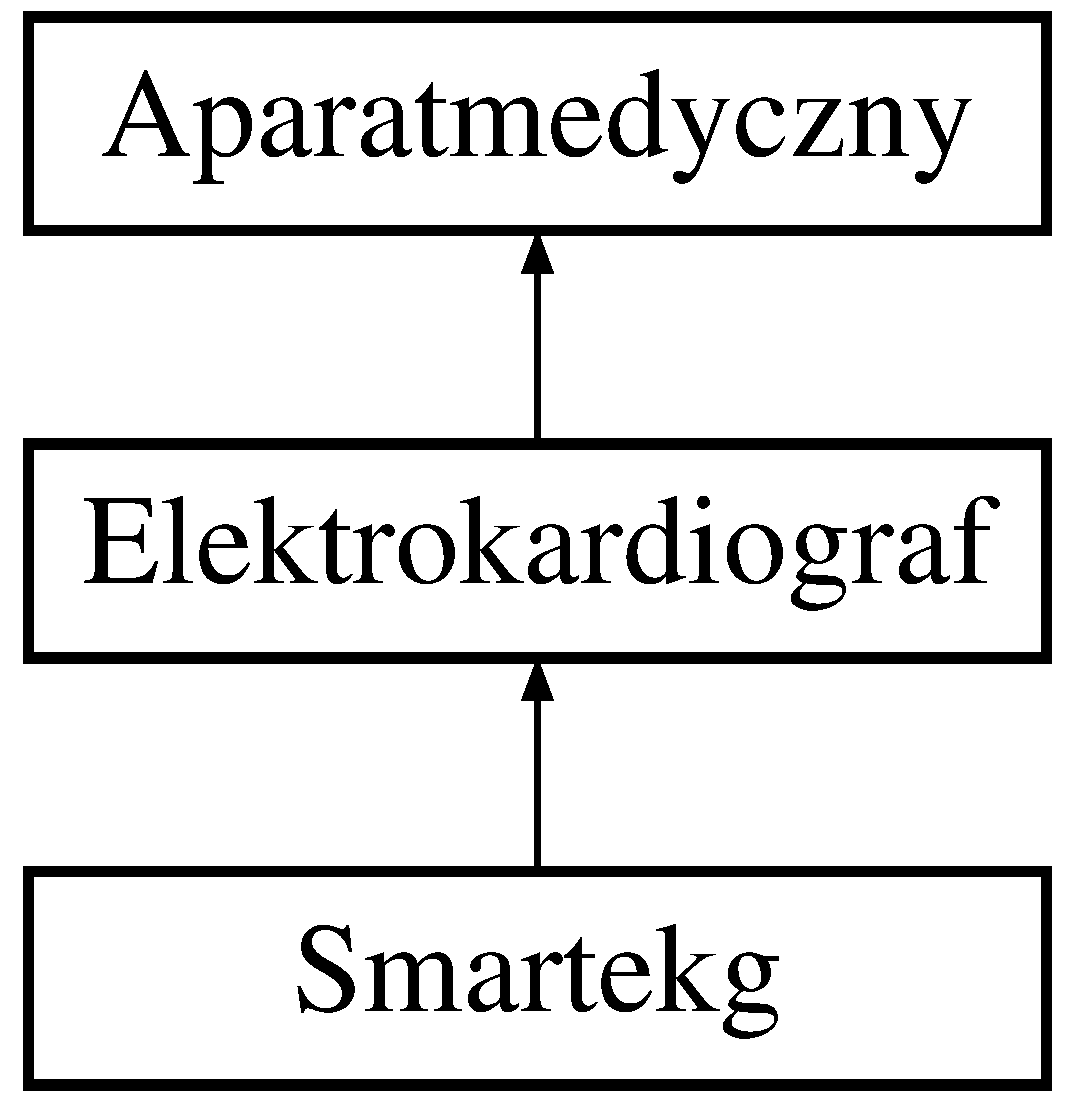
\includegraphics[height=3.000000cm]{class_smartekg}
\end{center}
\end{figure}
\subsection*{Public Member Functions}
\begin{DoxyCompactItemize}
\item 
\textbf{ Smartekg} ()
\begin{DoxyCompactList}\small\item\em konstruktor domyslny \end{DoxyCompactList}\item 
\textbf{ $\sim$\+Smartekg} ()
\begin{DoxyCompactList}\small\item\em destruktor domyslny \end{DoxyCompactList}\item 
void \textbf{ wlacz} ()
\begin{DoxyCompactList}\small\item\em wirtualna metoda wlaczenia przyrzadu \end{DoxyCompactList}\item 
void \textbf{ wylacz} ()
\begin{DoxyCompactList}\small\item\em wirtualna metoda wylaczenia przyrzadu \end{DoxyCompactList}\item 
void \textbf{ zrobbadanie} ()
\begin{DoxyCompactList}\small\item\em metoda \char`\"{}symulujaca\char`\"{} badania \end{DoxyCompactList}\item 
void \textbf{ ustaw} (bool, bool, bool)
\begin{DoxyCompactList}\small\item\em nadawanie parametrow \end{DoxyCompactList}\item 
void \textbf{ odczyt\+\_\+z\+\_\+pliku} (string)
\begin{DoxyCompactList}\small\item\em czytanie z pliku \end{DoxyCompactList}\item 
void \textbf{ zapisz\+\_\+do\+\_\+pliku} (string, int)
\begin{DoxyCompactList}\small\item\em zapisywanie do pliku \end{DoxyCompactList}\item 
void \textbf{ operator$<$$<$} (string s)
\begin{DoxyCompactList}\small\item\em operatory do zapisu w pliku przyjmujace jego nazwe \end{DoxyCompactList}\item 
void \textbf{ operator$>$$>$} (string s)
\begin{DoxyCompactList}\small\item\em operatory do odczytu z pliku przyjmujace jego nazwe \end{DoxyCompactList}\end{DoxyCompactItemize}
\subsection*{Friends}
\begin{DoxyCompactItemize}
\item 
ostream \& \textbf{ operator$<$$<$} (ostream \&wyjscie, const \textbf{ Smartekg} \&s)
\begin{DoxyCompactList}\small\item\em zaprzyjazniona funkcja do wypisania obiektu za pomoca cout \end{DoxyCompactList}\end{DoxyCompactItemize}
\subsection*{Additional Inherited Members}


\subsection{Detailed Description}
Klasa pochodna Elektrokardiografu. 

\subsection{Constructor \& Destructor Documentation}
\mbox{\label{class_smartekg_a82c28ed50e3117feea5f23c0cb9668ce}} 
\index{Smartekg@{Smartekg}!Smartekg@{Smartekg}}
\index{Smartekg@{Smartekg}!Smartekg@{Smartekg}}
\subsubsection{Smartekg()}
{\footnotesize\ttfamily Smartekg\+::\+Smartekg (\begin{DoxyParamCaption}{ }\end{DoxyParamCaption})}



konstruktor domyslny 

\mbox{\label{class_smartekg_afa82307ee5cad4bd96809ba1be9b4d3d}} 
\index{Smartekg@{Smartekg}!````~Smartekg@{$\sim$\+Smartekg}}
\index{````~Smartekg@{$\sim$\+Smartekg}!Smartekg@{Smartekg}}
\subsubsection{$\sim$\+Smartekg()}
{\footnotesize\ttfamily Smartekg\+::$\sim$\+Smartekg (\begin{DoxyParamCaption}{ }\end{DoxyParamCaption})}



destruktor domyslny 



\subsection{Member Function Documentation}
\mbox{\label{class_smartekg_a96fe1adb8c11601eefafe085ead3c3d1}} 
\index{Smartekg@{Smartekg}!odczyt\+\_\+z\+\_\+pliku@{odczyt\+\_\+z\+\_\+pliku}}
\index{odczyt\+\_\+z\+\_\+pliku@{odczyt\+\_\+z\+\_\+pliku}!Smartekg@{Smartekg}}
\subsubsection{odczyt\+\_\+z\+\_\+pliku()}
{\footnotesize\ttfamily void Smartekg\+::odczyt\+\_\+z\+\_\+pliku (\begin{DoxyParamCaption}\item[{string}]{s }\end{DoxyParamCaption})\hspace{0.3cm}{\ttfamily [virtual]}}



czytanie z pliku 


\begin{DoxyParams}{Parameters}
{\em string} & -\/ nazwa pliku \\
\hline
\end{DoxyParams}


Reimplemented from \textbf{ Elektrokardiograf} \doxyref{}{p.}{class_elektrokardiograf_af934c2d3456229093c37310070638df2}.

\mbox{\label{class_smartekg_ad4ebb0d3d69729f0ba0e04b066984713}} 
\index{Smartekg@{Smartekg}!operator$<$$<$@{operator$<$$<$}}
\index{operator$<$$<$@{operator$<$$<$}!Smartekg@{Smartekg}}
\subsubsection{operator$<$$<$()}
{\footnotesize\ttfamily void Smartekg\+::operator$<$$<$ (\begin{DoxyParamCaption}\item[{string}]{s }\end{DoxyParamCaption})}



operatory do zapisu w pliku przyjmujace jego nazwe 

\mbox{\label{class_smartekg_ac6898a9a2fc785c40211f2b1a5220534}} 
\index{Smartekg@{Smartekg}!operator$>$$>$@{operator$>$$>$}}
\index{operator$>$$>$@{operator$>$$>$}!Smartekg@{Smartekg}}
\subsubsection{operator$>$$>$()}
{\footnotesize\ttfamily void Smartekg\+::operator$>$$>$ (\begin{DoxyParamCaption}\item[{string}]{s }\end{DoxyParamCaption})}



operatory do odczytu z pliku przyjmujace jego nazwe 

\mbox{\label{class_smartekg_a1f3461e64d38bea214caaa157315be65}} 
\index{Smartekg@{Smartekg}!ustaw@{ustaw}}
\index{ustaw@{ustaw}!Smartekg@{Smartekg}}
\subsubsection{ustaw()}
{\footnotesize\ttfamily void Smartekg\+::ustaw (\begin{DoxyParamCaption}\item[{bool}]{blue,  }\item[{bool}]{net,  }\item[{bool}]{usb }\end{DoxyParamCaption})}



nadawanie parametrow 

\mbox{\label{class_smartekg_ab976b0a43ff21e254af74a29b4fc8688}} 
\index{Smartekg@{Smartekg}!wlacz@{wlacz}}
\index{wlacz@{wlacz}!Smartekg@{Smartekg}}
\subsubsection{wlacz()}
{\footnotesize\ttfamily void Smartekg\+::wlacz (\begin{DoxyParamCaption}{ }\end{DoxyParamCaption})\hspace{0.3cm}{\ttfamily [virtual]}}



wirtualna metoda wlaczenia przyrzadu 



Reimplemented from \textbf{ Elektrokardiograf} \doxyref{}{p.}{class_elektrokardiograf_a78b8311e31aa24ab92998e8105e72dd1}.

\mbox{\label{class_smartekg_a40cb07132a4139745bdf1cd31e2fd080}} 
\index{Smartekg@{Smartekg}!wylacz@{wylacz}}
\index{wylacz@{wylacz}!Smartekg@{Smartekg}}
\subsubsection{wylacz()}
{\footnotesize\ttfamily void Smartekg\+::wylacz (\begin{DoxyParamCaption}{ }\end{DoxyParamCaption})\hspace{0.3cm}{\ttfamily [virtual]}}



wirtualna metoda wylaczenia przyrzadu 



Reimplemented from \textbf{ Elektrokardiograf} \doxyref{}{p.}{class_elektrokardiograf_aea0ea515c89cddbdde78a2edef5dc34b}.

\mbox{\label{class_smartekg_afb055dc43e7012d04e8764507860ffad}} 
\index{Smartekg@{Smartekg}!zapisz\+\_\+do\+\_\+pliku@{zapisz\+\_\+do\+\_\+pliku}}
\index{zapisz\+\_\+do\+\_\+pliku@{zapisz\+\_\+do\+\_\+pliku}!Smartekg@{Smartekg}}
\subsubsection{zapisz\+\_\+do\+\_\+pliku()}
{\footnotesize\ttfamily void Smartekg\+::zapisz\+\_\+do\+\_\+pliku (\begin{DoxyParamCaption}\item[{string}]{s,  }\item[{int}]{zapis }\end{DoxyParamCaption})\hspace{0.3cm}{\ttfamily [virtual]}}



zapisywanie do pliku 


\begin{DoxyParams}{Parameters}
{\em string} & -\/ nazwa pliku \\
\hline
{\em int} & -\/ decyduje o dopisaniu do pliku lub nadpisaniu \\
\hline
\end{DoxyParams}


Reimplemented from \textbf{ Elektrokardiograf} \doxyref{}{p.}{class_elektrokardiograf_a7e9dc34e6867890ed9879bf5dcb5acfb}.

\mbox{\label{class_smartekg_a80a5495364b751184519215407ba8559}} 
\index{Smartekg@{Smartekg}!zrobbadanie@{zrobbadanie}}
\index{zrobbadanie@{zrobbadanie}!Smartekg@{Smartekg}}
\subsubsection{zrobbadanie()}
{\footnotesize\ttfamily void Smartekg\+::zrobbadanie (\begin{DoxyParamCaption}{ }\end{DoxyParamCaption})\hspace{0.3cm}{\ttfamily [virtual]}}



metoda \char`\"{}symulujaca\char`\"{} badania 



Reimplemented from \textbf{ Elektrokardiograf} \doxyref{}{p.}{class_elektrokardiograf_a4f43e5e6a427d074ee3a5acff7d96e14}.



\subsection{Friends And Related Function Documentation}
\mbox{\label{class_smartekg_a7d76f0593b32a68a973a114a28737c0d}} 
\index{Smartekg@{Smartekg}!operator$<$$<$@{operator$<$$<$}}
\index{operator$<$$<$@{operator$<$$<$}!Smartekg@{Smartekg}}
\subsubsection{operator$<$$<$}
{\footnotesize\ttfamily ostream\& operator$<$$<$ (\begin{DoxyParamCaption}\item[{ostream \&}]{wyjscie,  }\item[{const \textbf{ Smartekg} \&}]{s }\end{DoxyParamCaption})\hspace{0.3cm}{\ttfamily [friend]}}



zaprzyjazniona funkcja do wypisania obiektu za pomoca cout 



The documentation for this class was generated from the following files\+:\begin{DoxyCompactItemize}
\item 
\textbf{ smartekg.\+h}\item 
\textbf{ smartekg.\+cpp}\end{DoxyCompactItemize}

\section{Termometr Class Reference}
\label{class_termometr}\index{Termometr@{Termometr}}


\doxyref{Termometr}{p.}{class_termometr} ,dziedziczacy po klasie \doxyref{Aparatmedyczny}{p.}{class_aparatmedyczny}.  




{\ttfamily \#include $<$termometr.\+h$>$}

Inheritance diagram for Termometr\+:\begin{figure}[H]
\begin{center}
\leavevmode
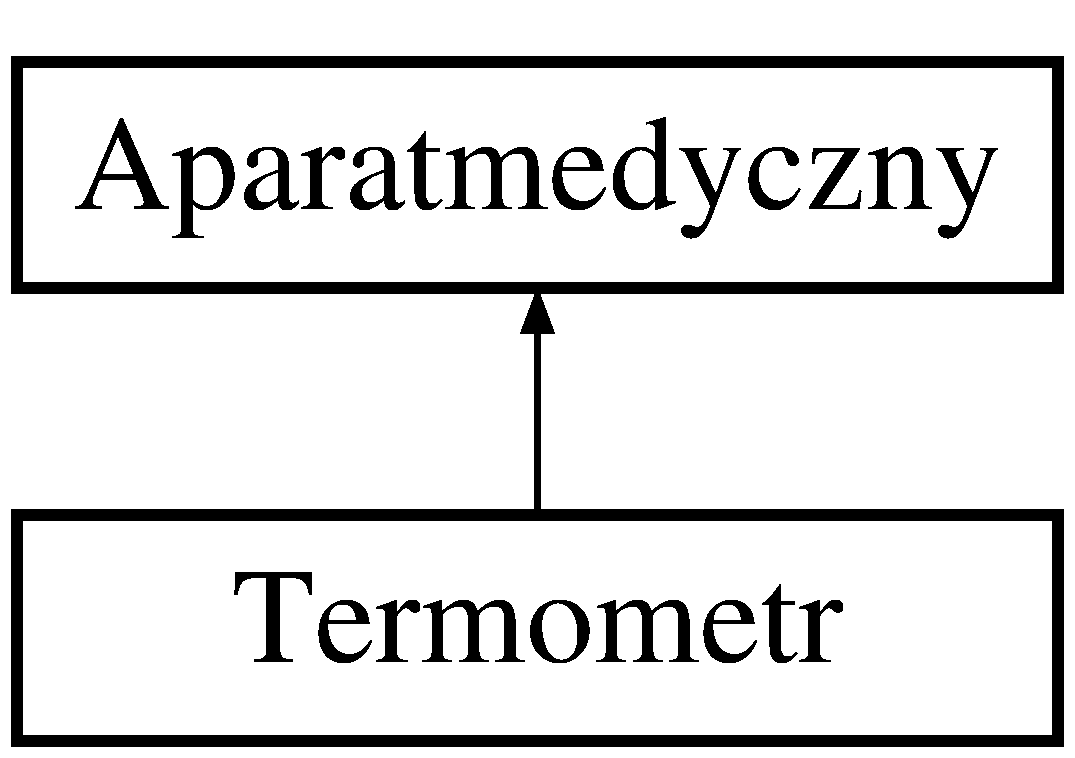
\includegraphics[height=2.000000cm]{class_termometr}
\end{center}
\end{figure}
\subsection*{Public Member Functions}
\begin{DoxyCompactItemize}
\item 
void \textbf{ wlacz} ()
\begin{DoxyCompactList}\small\item\em wirtualna metoda wlaczenia przyrzadu \end{DoxyCompactList}\item 
void \textbf{ wylacz} ()
\begin{DoxyCompactList}\small\item\em wirtualna metoda wylaczenia przyrzadu \end{DoxyCompactList}\item 
void \textbf{ zrobbadanie} ()
\begin{DoxyCompactList}\small\item\em metoda \char`\"{}symulujaca\char`\"{} badania \end{DoxyCompactList}\item 
void \textbf{ uzupelnij\+\_\+dane} (int, double, double, double, int, string)
\begin{DoxyCompactList}\small\item\em nadawanie parametrow \end{DoxyCompactList}\item 
\textbf{ Termometr} ()
\begin{DoxyCompactList}\small\item\em konstruktor domyslny \end{DoxyCompactList}\item 
\textbf{ Termometr} (int, bool, string)
\begin{DoxyCompactList}\small\item\em konstruktor z parametrami \end{DoxyCompactList}\item 
\textbf{ $\sim$\+Termometr} ()
\begin{DoxyCompactList}\small\item\em destruktor \end{DoxyCompactList}\item 
void \textbf{ odczyt\+\_\+z\+\_\+pliku} (string)
\begin{DoxyCompactList}\small\item\em czytanie z pliku \end{DoxyCompactList}\item 
void \textbf{ zapisz\+\_\+do\+\_\+pliku} (string, int)
\begin{DoxyCompactList}\small\item\em zapisywanie do pliku \end{DoxyCompactList}\item 
void \textbf{ operator$<$$<$} (string s)
\begin{DoxyCompactList}\small\item\em operatory do zapisu w pliku przyjmujace jego nazwe \end{DoxyCompactList}\item 
void \textbf{ operator$>$$>$} (string s)
\begin{DoxyCompactList}\small\item\em operatory do odczytu z pliku przyjmujace jego nazwe \end{DoxyCompactList}\end{DoxyCompactItemize}
\subsection*{Friends}
\begin{DoxyCompactItemize}
\item 
ostream \& \textbf{ operator$<$$<$} (ostream \&wyjscie, const \textbf{ Termometr} \&s)
\begin{DoxyCompactList}\small\item\em zaprzyjazniona funkcja do wypisania obiektu za pomoca cout \end{DoxyCompactList}\end{DoxyCompactItemize}
\subsection*{Additional Inherited Members}


\subsection{Detailed Description}
\doxyref{Termometr}{p.}{class_termometr} ,dziedziczacy po klasie \doxyref{Aparatmedyczny}{p.}{class_aparatmedyczny}. 

\subsection{Constructor \& Destructor Documentation}
\mbox{\label{class_termometr_a73dfb1aef59ff906433c0966728ca8f1}} 
\index{Termometr@{Termometr}!Termometr@{Termometr}}
\index{Termometr@{Termometr}!Termometr@{Termometr}}
\subsubsection{Termometr()\hspace{0.1cm}{\footnotesize\ttfamily [1/2]}}
{\footnotesize\ttfamily Termometr\+::\+Termometr (\begin{DoxyParamCaption}{ }\end{DoxyParamCaption})}



konstruktor domyslny 

\mbox{\label{class_termometr_a6a5981fa5ff2bd1545121241ae5c0c6c}} 
\index{Termometr@{Termometr}!Termometr@{Termometr}}
\index{Termometr@{Termometr}!Termometr@{Termometr}}
\subsubsection{Termometr()\hspace{0.1cm}{\footnotesize\ttfamily [2/2]}}
{\footnotesize\ttfamily Termometr\+::\+Termometr (\begin{DoxyParamCaption}\item[{int}]{czas,  }\item[{bool}]{dz,  }\item[{string}]{mod }\end{DoxyParamCaption})}



konstruktor z parametrami 

\mbox{\label{class_termometr_ac388fb0a0ebba9a70fa620c43da6cc56}} 
\index{Termometr@{Termometr}!````~Termometr@{$\sim$\+Termometr}}
\index{````~Termometr@{$\sim$\+Termometr}!Termometr@{Termometr}}
\subsubsection{$\sim$\+Termometr()}
{\footnotesize\ttfamily Termometr\+::$\sim$\+Termometr (\begin{DoxyParamCaption}{ }\end{DoxyParamCaption})}



destruktor 



\subsection{Member Function Documentation}
\mbox{\label{class_termometr_a42a1dab82d6f7c1adba8b03b01d132d8}} 
\index{Termometr@{Termometr}!odczyt\+\_\+z\+\_\+pliku@{odczyt\+\_\+z\+\_\+pliku}}
\index{odczyt\+\_\+z\+\_\+pliku@{odczyt\+\_\+z\+\_\+pliku}!Termometr@{Termometr}}
\subsubsection{odczyt\+\_\+z\+\_\+pliku()}
{\footnotesize\ttfamily void Termometr\+::odczyt\+\_\+z\+\_\+pliku (\begin{DoxyParamCaption}\item[{string}]{s }\end{DoxyParamCaption})\hspace{0.3cm}{\ttfamily [virtual]}}



czytanie z pliku 


\begin{DoxyParams}{Parameters}
{\em string} & -\/ nazwa pliku \\
\hline
\end{DoxyParams}


Implements \textbf{ Aparatmedyczny} \doxyref{}{p.}{class_aparatmedyczny_a5300ce8466293b738da4f2eb5ed7b233}.

\mbox{\label{class_termometr_ae3759a51f581779a5b61efa447534a58}} 
\index{Termometr@{Termometr}!operator$<$$<$@{operator$<$$<$}}
\index{operator$<$$<$@{operator$<$$<$}!Termometr@{Termometr}}
\subsubsection{operator$<$$<$()}
{\footnotesize\ttfamily void Termometr\+::operator$<$$<$ (\begin{DoxyParamCaption}\item[{string}]{s }\end{DoxyParamCaption})}



operatory do zapisu w pliku przyjmujace jego nazwe 

\mbox{\label{class_termometr_a96f6e3d168dd905e6f5900bbbf66fc94}} 
\index{Termometr@{Termometr}!operator$>$$>$@{operator$>$$>$}}
\index{operator$>$$>$@{operator$>$$>$}!Termometr@{Termometr}}
\subsubsection{operator$>$$>$()}
{\footnotesize\ttfamily void Termometr\+::operator$>$$>$ (\begin{DoxyParamCaption}\item[{string}]{s }\end{DoxyParamCaption})}



operatory do odczytu z pliku przyjmujace jego nazwe 

\mbox{\label{class_termometr_a67bdf95b9163faf32c5261abf13e7b0b}} 
\index{Termometr@{Termometr}!uzupelnij\+\_\+dane@{uzupelnij\+\_\+dane}}
\index{uzupelnij\+\_\+dane@{uzupelnij\+\_\+dane}!Termometr@{Termometr}}
\subsubsection{uzupelnij\+\_\+dane()}
{\footnotesize\ttfamily void Termometr\+::uzupelnij\+\_\+dane (\begin{DoxyParamCaption}\item[{int}]{qw,  }\item[{double}]{we,  }\item[{double}]{er,  }\item[{double}]{rt,  }\item[{int}]{a,  }\item[{string}]{c }\end{DoxyParamCaption})}



nadawanie parametrow 

Parametry to kolejno atrybuty obiektu tej klasy \mbox{\label{class_termometr_a25df4488ebce81d7c92d2c66ca02fb6d}} 
\index{Termometr@{Termometr}!wlacz@{wlacz}}
\index{wlacz@{wlacz}!Termometr@{Termometr}}
\subsubsection{wlacz()}
{\footnotesize\ttfamily void Termometr\+::wlacz (\begin{DoxyParamCaption}{ }\end{DoxyParamCaption})\hspace{0.3cm}{\ttfamily [virtual]}}



wirtualna metoda wlaczenia przyrzadu 



Implements \textbf{ Aparatmedyczny} \doxyref{}{p.}{class_aparatmedyczny_a303cd2ab42aa4a4a29bb59d685573c78}.

\mbox{\label{class_termometr_ac13dc274e2f18f76ff8c1eb60f793a20}} 
\index{Termometr@{Termometr}!wylacz@{wylacz}}
\index{wylacz@{wylacz}!Termometr@{Termometr}}
\subsubsection{wylacz()}
{\footnotesize\ttfamily void Termometr\+::wylacz (\begin{DoxyParamCaption}{ }\end{DoxyParamCaption})\hspace{0.3cm}{\ttfamily [virtual]}}



wirtualna metoda wylaczenia przyrzadu 



Implements \textbf{ Aparatmedyczny} \doxyref{}{p.}{class_aparatmedyczny_a0f6e8f2d4656bc258805e230ad4563d0}.

\mbox{\label{class_termometr_a852973a522848a9fbbd95361494525a4}} 
\index{Termometr@{Termometr}!zapisz\+\_\+do\+\_\+pliku@{zapisz\+\_\+do\+\_\+pliku}}
\index{zapisz\+\_\+do\+\_\+pliku@{zapisz\+\_\+do\+\_\+pliku}!Termometr@{Termometr}}
\subsubsection{zapisz\+\_\+do\+\_\+pliku()}
{\footnotesize\ttfamily void Termometr\+::zapisz\+\_\+do\+\_\+pliku (\begin{DoxyParamCaption}\item[{string}]{s,  }\item[{int}]{zapis }\end{DoxyParamCaption})\hspace{0.3cm}{\ttfamily [virtual]}}



zapisywanie do pliku 


\begin{DoxyParams}{Parameters}
{\em string} & -\/ nazwa pliku \\
\hline
{\em int} & -\/ decyduje o dopisaniu do pliku lub nadpisaniu \\
\hline
\end{DoxyParams}


Implements \textbf{ Aparatmedyczny} \doxyref{}{p.}{class_aparatmedyczny_aa81d3a1b324550cd90fba34d1096f772}.

\mbox{\label{class_termometr_acd74b1f25bb4af260d5f4f9d6baf4921}} 
\index{Termometr@{Termometr}!zrobbadanie@{zrobbadanie}}
\index{zrobbadanie@{zrobbadanie}!Termometr@{Termometr}}
\subsubsection{zrobbadanie()}
{\footnotesize\ttfamily void Termometr\+::zrobbadanie (\begin{DoxyParamCaption}{ }\end{DoxyParamCaption})\hspace{0.3cm}{\ttfamily [virtual]}}



metoda \char`\"{}symulujaca\char`\"{} badania 



Implements \textbf{ Aparatmedyczny} \doxyref{}{p.}{class_aparatmedyczny_adbdf7a6290c67862387d1cda2f0d9173}.



\subsection{Friends And Related Function Documentation}
\mbox{\label{class_termometr_aa076a790576f7719b5dba864120a1b44}} 
\index{Termometr@{Termometr}!operator$<$$<$@{operator$<$$<$}}
\index{operator$<$$<$@{operator$<$$<$}!Termometr@{Termometr}}
\subsubsection{operator$<$$<$}
{\footnotesize\ttfamily ostream\& operator$<$$<$ (\begin{DoxyParamCaption}\item[{ostream \&}]{wyjscie,  }\item[{const \textbf{ Termometr} \&}]{s }\end{DoxyParamCaption})\hspace{0.3cm}{\ttfamily [friend]}}



zaprzyjazniona funkcja do wypisania obiektu za pomoca cout 



The documentation for this class was generated from the following files\+:\begin{DoxyCompactItemize}
\item 
\textbf{ termometr.\+h}\item 
\textbf{ termometr.\+cpp}\end{DoxyCompactItemize}

\section{Wyswietlacz Class Reference}
\label{class_wyswietlacz}\index{Wyswietlacz@{Wyswietlacz}}


Podobiekt Elektrokardigrafu i \doxyref{Smartekg}{p.}{class_smartekg}.  




{\ttfamily \#include $<$wyswietlacz.\+h$>$}

\subsection*{Public Member Functions}
\begin{DoxyCompactItemize}
\item 
\textbf{ Wyswietlacz} ()
\begin{DoxyCompactList}\small\item\em konstruktor domyslny \end{DoxyCompactList}\item 
void \textbf{ uzupelnij\+\_\+dane} (int, int, int, bool, string)
\begin{DoxyCompactList}\small\item\em nadawanie parametrow \end{DoxyCompactList}\item 
\textbf{ $\sim$\+Wyswietlacz} ()
\begin{DoxyCompactList}\small\item\em destruktor wyswietlacza \end{DoxyCompactList}\item 
void \textbf{ odczyt\+\_\+z\+\_\+pliku} (string)
\begin{DoxyCompactList}\small\item\em czytanie z pliku \end{DoxyCompactList}\item 
void \textbf{ zapisz\+\_\+do\+\_\+pliku} (string, int)
\begin{DoxyCompactList}\small\item\em zapisywanie do pliku \end{DoxyCompactList}\item 
void \textbf{ operator$<$$<$} (string s)
\begin{DoxyCompactList}\small\item\em operatory do zapisu w pliku przyjmujace jego nazwe \end{DoxyCompactList}\item 
void \textbf{ operator$>$$>$} (string s)
\begin{DoxyCompactList}\small\item\em operatory do odczytu z pliku przyjmujace jego nazwe \end{DoxyCompactList}\end{DoxyCompactItemize}
\subsection*{Friends}
\begin{DoxyCompactItemize}
\item 
ostream \& \textbf{ operator$<$$<$} (ostream \&wyjscie, const \textbf{ Wyswietlacz} \&s)
\begin{DoxyCompactList}\small\item\em zaprzyjazniona funkcja do wypisania obiektu za pomoca cout \end{DoxyCompactList}\end{DoxyCompactItemize}


\subsection{Detailed Description}
Podobiekt Elektrokardigrafu i \doxyref{Smartekg}{p.}{class_smartekg}. 

\subsection{Constructor \& Destructor Documentation}
\mbox{\label{class_wyswietlacz_a184f33d2f0e1070e5bb3a7b7d35d152f}} 
\index{Wyswietlacz@{Wyswietlacz}!Wyswietlacz@{Wyswietlacz}}
\index{Wyswietlacz@{Wyswietlacz}!Wyswietlacz@{Wyswietlacz}}
\subsubsection{Wyswietlacz()}
{\footnotesize\ttfamily Wyswietlacz\+::\+Wyswietlacz (\begin{DoxyParamCaption}{ }\end{DoxyParamCaption})}



konstruktor domyslny 

\mbox{\label{class_wyswietlacz_a24b579830d186f91f23cf539575695c7}} 
\index{Wyswietlacz@{Wyswietlacz}!````~Wyswietlacz@{$\sim$\+Wyswietlacz}}
\index{````~Wyswietlacz@{$\sim$\+Wyswietlacz}!Wyswietlacz@{Wyswietlacz}}
\subsubsection{$\sim$\+Wyswietlacz()}
{\footnotesize\ttfamily Wyswietlacz\+::$\sim$\+Wyswietlacz (\begin{DoxyParamCaption}{ }\end{DoxyParamCaption})}



destruktor wyswietlacza 



\subsection{Member Function Documentation}
\mbox{\label{class_wyswietlacz_ab4a83e1fa18beb664003cd0d11980935}} 
\index{Wyswietlacz@{Wyswietlacz}!odczyt\+\_\+z\+\_\+pliku@{odczyt\+\_\+z\+\_\+pliku}}
\index{odczyt\+\_\+z\+\_\+pliku@{odczyt\+\_\+z\+\_\+pliku}!Wyswietlacz@{Wyswietlacz}}
\subsubsection{odczyt\+\_\+z\+\_\+pliku()}
{\footnotesize\ttfamily void Wyswietlacz\+::odczyt\+\_\+z\+\_\+pliku (\begin{DoxyParamCaption}\item[{string}]{s }\end{DoxyParamCaption})}



czytanie z pliku 


\begin{DoxyParams}{Parameters}
{\em string} & -\/ nazwa pliku \\
\hline
\end{DoxyParams}
\mbox{\label{class_wyswietlacz_a9ed051469a93130fba9c6ac107954fdf}} 
\index{Wyswietlacz@{Wyswietlacz}!operator$<$$<$@{operator$<$$<$}}
\index{operator$<$$<$@{operator$<$$<$}!Wyswietlacz@{Wyswietlacz}}
\subsubsection{operator$<$$<$()}
{\footnotesize\ttfamily void Wyswietlacz\+::operator$<$$<$ (\begin{DoxyParamCaption}\item[{string}]{s }\end{DoxyParamCaption})}



operatory do zapisu w pliku przyjmujace jego nazwe 

\mbox{\label{class_wyswietlacz_a7e41ea08f95671c9cc0ed1fb046aa6e4}} 
\index{Wyswietlacz@{Wyswietlacz}!operator$>$$>$@{operator$>$$>$}}
\index{operator$>$$>$@{operator$>$$>$}!Wyswietlacz@{Wyswietlacz}}
\subsubsection{operator$>$$>$()}
{\footnotesize\ttfamily void Wyswietlacz\+::operator$>$$>$ (\begin{DoxyParamCaption}\item[{string}]{s }\end{DoxyParamCaption})}



operatory do odczytu z pliku przyjmujace jego nazwe 

\mbox{\label{class_wyswietlacz_ae5091e734c19e2f537bd374c4e7ae4e5}} 
\index{Wyswietlacz@{Wyswietlacz}!uzupelnij\+\_\+dane@{uzupelnij\+\_\+dane}}
\index{uzupelnij\+\_\+dane@{uzupelnij\+\_\+dane}!Wyswietlacz@{Wyswietlacz}}
\subsubsection{uzupelnij\+\_\+dane()}
{\footnotesize\ttfamily void Wyswietlacz\+::uzupelnij\+\_\+dane (\begin{DoxyParamCaption}\item[{int}]{a,  }\item[{int}]{b,  }\item[{int}]{c,  }\item[{bool}]{d,  }\item[{string}]{e }\end{DoxyParamCaption})}



nadawanie parametrow 

Parametry to kolejno atrybuty obiektu tej klasy \mbox{\label{class_wyswietlacz_aa44dac8ae7a0a84549a08e9042db1746}} 
\index{Wyswietlacz@{Wyswietlacz}!zapisz\+\_\+do\+\_\+pliku@{zapisz\+\_\+do\+\_\+pliku}}
\index{zapisz\+\_\+do\+\_\+pliku@{zapisz\+\_\+do\+\_\+pliku}!Wyswietlacz@{Wyswietlacz}}
\subsubsection{zapisz\+\_\+do\+\_\+pliku()}
{\footnotesize\ttfamily void Wyswietlacz\+::zapisz\+\_\+do\+\_\+pliku (\begin{DoxyParamCaption}\item[{string}]{s,  }\item[{int}]{zapis }\end{DoxyParamCaption})}



zapisywanie do pliku 


\begin{DoxyParams}{Parameters}
{\em string} & -\/ nazwa pliku \\
\hline
{\em int} & -\/ decyduje o dopisaniu do pliku lub nadpisaniu \\
\hline
\end{DoxyParams}


\subsection{Friends And Related Function Documentation}
\mbox{\label{class_wyswietlacz_ae6d943d6ec6cf596444b451cb978e07f}} 
\index{Wyswietlacz@{Wyswietlacz}!operator$<$$<$@{operator$<$$<$}}
\index{operator$<$$<$@{operator$<$$<$}!Wyswietlacz@{Wyswietlacz}}
\subsubsection{operator$<$$<$}
{\footnotesize\ttfamily ostream\& operator$<$$<$ (\begin{DoxyParamCaption}\item[{ostream \&}]{wyjscie,  }\item[{const \textbf{ Wyswietlacz} \&}]{s }\end{DoxyParamCaption})\hspace{0.3cm}{\ttfamily [friend]}}



zaprzyjazniona funkcja do wypisania obiektu za pomoca cout 



The documentation for this class was generated from the following files\+:\begin{DoxyCompactItemize}
\item 
\textbf{ wyswietlacz.\+h}\item 
\textbf{ wyswietlacz.\+cpp}\end{DoxyCompactItemize}

\chapter{File Documentation}
\section{aparatmedyczny.\+h File Reference}
\label{aparatmedyczny_8h}\index{aparatmedyczny.\+h@{aparatmedyczny.\+h}}
{\ttfamily \#include $<$iostream$>$}\newline
{\ttfamily \#include $<$string$>$}\newline
\subsection*{Classes}
\begin{DoxyCompactItemize}
\item 
class \textbf{ Aparatmedyczny}
\begin{DoxyCompactList}\small\item\em klasas wirtualna \end{DoxyCompactList}\end{DoxyCompactItemize}

\section{bateria.\+cpp File Reference}
\label{bateria_8cpp}\index{bateria.\+cpp@{bateria.\+cpp}}
{\ttfamily \#include \char`\"{}bateria.\+h\char`\"{}}\newline
\subsection*{Functions}
\begin{DoxyCompactItemize}
\item 
ostream \& \textbf{ operator$<$$<$} (ostream \&wyjscie, const \textbf{ Bateria} \&s)
\end{DoxyCompactItemize}


\subsection{Function Documentation}
\mbox{\label{bateria_8cpp_a47035e47d5dc1f14ae25b6033bf175dc}} 
\index{bateria.\+cpp@{bateria.\+cpp}!operator$<$$<$@{operator$<$$<$}}
\index{operator$<$$<$@{operator$<$$<$}!bateria.\+cpp@{bateria.\+cpp}}
\subsubsection{operator$<$$<$()}
{\footnotesize\ttfamily ostream\& operator$<$$<$ (\begin{DoxyParamCaption}\item[{ostream \&}]{wyjscie,  }\item[{const \textbf{ Bateria} \&}]{s }\end{DoxyParamCaption})}


\section{bateria.\+h File Reference}
\label{bateria_8h}\index{bateria.\+h@{bateria.\+h}}
{\ttfamily \#include $<$string$>$}\newline
{\ttfamily \#include $<$iostream$>$}\newline
{\ttfamily \#include $<$fstream$>$}\newline
\subsection*{Classes}
\begin{DoxyCompactItemize}
\item 
class \textbf{ Bateria}
\begin{DoxyCompactList}\small\item\em \doxyref{Bateria}{p.}{class_bateria} podobiekt E\+KG. \end{DoxyCompactList}\end{DoxyCompactItemize}

\section{drukarka.\+cpp File Reference}
\label{drukarka_8cpp}\index{drukarka.\+cpp@{drukarka.\+cpp}}
{\ttfamily \#include \char`\"{}drukarka.\+h\char`\"{}}\newline

\section{drukarka.\+h File Reference}
\label{drukarka_8h}\index{drukarka.\+h@{drukarka.\+h}}
{\ttfamily \#include $<$string$>$}\newline
{\ttfamily \#include $<$iostream$>$}\newline
{\ttfamily \#include $<$fstream$>$}\newline
{\ttfamily \#include $<$queue$>$}\newline
\subsection*{Classes}
\begin{DoxyCompactItemize}
\item 
class \textbf{ Drukarka}
\begin{DoxyCompactList}\small\item\em Podobiekt Elektrokardiografu. \end{DoxyCompactList}\end{DoxyCompactItemize}

\section{elektrokardiograf.\+cpp File Reference}
\label{elektrokardiograf_8cpp}\index{elektrokardiograf.\+cpp@{elektrokardiograf.\+cpp}}
{\ttfamily \#include \char`\"{}elektrokardiograf.\+h\char`\"{}}\newline
\subsection*{Functions}
\begin{DoxyCompactItemize}
\item 
ostream \& \textbf{ operator$<$$<$} (ostream \&wyjscie, const \textbf{ Elektrokardiograf} \&s)
\end{DoxyCompactItemize}


\subsection{Function Documentation}
\mbox{\label{elektrokardiograf_8cpp_a10836bab7baab06a7a2a5d276b1eee15}} 
\index{elektrokardiograf.\+cpp@{elektrokardiograf.\+cpp}!operator$<$$<$@{operator$<$$<$}}
\index{operator$<$$<$@{operator$<$$<$}!elektrokardiograf.\+cpp@{elektrokardiograf.\+cpp}}
\subsubsection{operator$<$$<$()}
{\footnotesize\ttfamily ostream\& operator$<$$<$ (\begin{DoxyParamCaption}\item[{ostream \&}]{wyjscie,  }\item[{const \textbf{ Elektrokardiograf} \&}]{s }\end{DoxyParamCaption})}


\section{elektrokardiograf.\+h File Reference}
\label{elektrokardiograf_8h}\index{elektrokardiograf.\+h@{elektrokardiograf.\+h}}
{\ttfamily \#include \char`\"{}bateria.\+h\char`\"{}}\newline
{\ttfamily \#include \char`\"{}drukarka.\+h\char`\"{}}\newline
{\ttfamily \#include \char`\"{}aparatmedyczny.\+h\char`\"{}}\newline
{\ttfamily \#include \char`\"{}wyswietlacz.\+h\char`\"{}}\newline
\subsection*{Classes}
\begin{DoxyCompactItemize}
\item 
class \textbf{ Elektrokardiograf}
\begin{DoxyCompactList}\small\item\em klasa \doxyref{Elektrokardiograf}{p.}{class_elektrokardiograf} obiekt glowny dziedziczaca po \doxyref{Aparatmedyczny}{p.}{class_aparatmedyczny} \end{DoxyCompactList}\end{DoxyCompactItemize}

\section{interfejs.\+cpp File Reference}
\label{interfejs_8cpp}\index{interfejs.\+cpp@{interfejs.\+cpp}}
{\ttfamily \#include $<$conio.\+h$>$}\newline
{\ttfamily \#include \char`\"{}interfejs.\+h\char`\"{}}\newline
\subsection*{Functions}
\begin{DoxyCompactItemize}
\item 
void \textbf{ interfejs} ()
\begin{DoxyCompactList}\small\item\em funkcja symulujaca interfejs \end{DoxyCompactList}\end{DoxyCompactItemize}


\subsection{Function Documentation}
\mbox{\label{interfejs_8cpp_a3105c716b75322c6bbec3dfa0a457125}} 
\index{interfejs.\+cpp@{interfejs.\+cpp}!interfejs@{interfejs}}
\index{interfejs@{interfejs}!interfejs.\+cpp@{interfejs.\+cpp}}
\subsubsection{interfejs()}
{\footnotesize\ttfamily void interfejs (\begin{DoxyParamCaption}{ }\end{DoxyParamCaption})}



funkcja symulujaca interfejs 


\section{interfejs.\+h File Reference}
\label{interfejs_8h}\index{interfejs.\+h@{interfejs.\+h}}
{\ttfamily \#include \char`\"{}smartekg.\+h\char`\"{}}\newline
{\ttfamily \#include \char`\"{}termometr.\+h\char`\"{}}\newline
\subsection*{Functions}
\begin{DoxyCompactItemize}
\item 
void \textbf{ interfejs} ()
\begin{DoxyCompactList}\small\item\em funkcja symulujaca interfejs \end{DoxyCompactList}\end{DoxyCompactItemize}


\subsection{Function Documentation}
\mbox{\label{interfejs_8h_a3105c716b75322c6bbec3dfa0a457125}} 
\index{interfejs.\+h@{interfejs.\+h}!interfejs@{interfejs}}
\index{interfejs@{interfejs}!interfejs.\+h@{interfejs.\+h}}
\subsubsection{interfejs()}
{\footnotesize\ttfamily void interfejs (\begin{DoxyParamCaption}{ }\end{DoxyParamCaption})}



funkcja symulujaca interfejs 


\section{main.\+cpp File Reference}
\label{main_8cpp}\index{main.\+cpp@{main.\+cpp}}
{\ttfamily \#include $<$iostream$>$}\newline
{\ttfamily \#include $<$string$>$}\newline
{\ttfamily \#include \char`\"{}interfejs.\+h\char`\"{}}\newline
\subsection*{Functions}
\begin{DoxyCompactItemize}
\item 
int \textbf{ main} ()
\end{DoxyCompactItemize}


\subsection{Function Documentation}
\mbox{\label{main_8cpp_ae66f6b31b5ad750f1fe042a706a4e3d4}} 
\index{main.\+cpp@{main.\+cpp}!main@{main}}
\index{main@{main}!main.\+cpp@{main.\+cpp}}
\subsubsection{main()}
{\footnotesize\ttfamily int main (\begin{DoxyParamCaption}{ }\end{DoxyParamCaption})}


\section{smartekg.\+cpp File Reference}
\label{smartekg_8cpp}\index{smartekg.\+cpp@{smartekg.\+cpp}}
{\ttfamily \#include \char`\"{}smartekg.\+h\char`\"{}}\newline
\subsection*{Functions}
\begin{DoxyCompactItemize}
\item 
ostream \& \textbf{ operator$<$$<$} (ostream \&wyjscie, const \textbf{ Smartekg} \&s)
\end{DoxyCompactItemize}


\subsection{Function Documentation}
\mbox{\label{smartekg_8cpp_a7d76f0593b32a68a973a114a28737c0d}} 
\index{smartekg.\+cpp@{smartekg.\+cpp}!operator$<$$<$@{operator$<$$<$}}
\index{operator$<$$<$@{operator$<$$<$}!smartekg.\+cpp@{smartekg.\+cpp}}
\subsubsection{operator$<$$<$()}
{\footnotesize\ttfamily ostream\& operator$<$$<$ (\begin{DoxyParamCaption}\item[{ostream \&}]{wyjscie,  }\item[{const \textbf{ Smartekg} \&}]{s }\end{DoxyParamCaption})}


\section{smartekg.\+h File Reference}
\label{smartekg_8h}\index{smartekg.\+h@{smartekg.\+h}}
{\ttfamily \#include \char`\"{}elektrokardiograf.\+h\char`\"{}}\newline
\subsection*{Classes}
\begin{DoxyCompactItemize}
\item 
class \textbf{ Smartekg}
\begin{DoxyCompactList}\small\item\em Klasa pochodna Elektrokardiografu. \end{DoxyCompactList}\end{DoxyCompactItemize}

\section{termometr.\+cpp File Reference}
\label{termometr_8cpp}\index{termometr.\+cpp@{termometr.\+cpp}}
{\ttfamily \#include \char`\"{}termometr.\+h\char`\"{}}\newline
\subsection*{Functions}
\begin{DoxyCompactItemize}
\item 
ostream \& \textbf{ operator$<$$<$} (ostream \&wyjscie, const \textbf{ Termometr} \&s)
\end{DoxyCompactItemize}


\subsection{Function Documentation}
\mbox{\label{termometr_8cpp_aa076a790576f7719b5dba864120a1b44}} 
\index{termometr.\+cpp@{termometr.\+cpp}!operator$<$$<$@{operator$<$$<$}}
\index{operator$<$$<$@{operator$<$$<$}!termometr.\+cpp@{termometr.\+cpp}}
\subsubsection{operator$<$$<$()}
{\footnotesize\ttfamily ostream\& operator$<$$<$ (\begin{DoxyParamCaption}\item[{ostream \&}]{wyjscie,  }\item[{const \textbf{ Termometr} \&}]{s }\end{DoxyParamCaption})}


\section{termometr.\+h File Reference}
\label{termometr_8h}\index{termometr.\+h@{termometr.\+h}}
{\ttfamily \#include $<$iostream$>$}\newline
{\ttfamily \#include $<$string$>$}\newline
{\ttfamily \#include $<$fstream$>$}\newline
{\ttfamily \#include \char`\"{}aparatmedyczny.\+h\char`\"{}}\newline
\subsection*{Classes}
\begin{DoxyCompactItemize}
\item 
class \textbf{ Termometr}
\begin{DoxyCompactList}\small\item\em \doxyref{Termometr}{p.}{class_termometr} ,dziedziczacy po klasie \doxyref{Aparatmedyczny}{p.}{class_aparatmedyczny}. \end{DoxyCompactList}\end{DoxyCompactItemize}

\section{wyswietlacz.\+cpp File Reference}
\label{wyswietlacz_8cpp}\index{wyswietlacz.\+cpp@{wyswietlacz.\+cpp}}
{\ttfamily \#include \char`\"{}wyswietlacz.\+h\char`\"{}}\newline
\subsection*{Functions}
\begin{DoxyCompactItemize}
\item 
ostream \& \textbf{ operator$<$$<$} (ostream \&wyjscie, const \textbf{ Wyswietlacz} \&s)
\end{DoxyCompactItemize}


\subsection{Function Documentation}
\mbox{\label{wyswietlacz_8cpp_ae6d943d6ec6cf596444b451cb978e07f}} 
\index{wyswietlacz.\+cpp@{wyswietlacz.\+cpp}!operator$<$$<$@{operator$<$$<$}}
\index{operator$<$$<$@{operator$<$$<$}!wyswietlacz.\+cpp@{wyswietlacz.\+cpp}}
\subsubsection{operator$<$$<$()}
{\footnotesize\ttfamily ostream\& operator$<$$<$ (\begin{DoxyParamCaption}\item[{ostream \&}]{wyjscie,  }\item[{const \textbf{ Wyswietlacz} \&}]{s }\end{DoxyParamCaption})}


\section{wyswietlacz.\+h File Reference}
\label{wyswietlacz_8h}\index{wyswietlacz.\+h@{wyswietlacz.\+h}}
{\ttfamily \#include $<$string$>$}\newline
{\ttfamily \#include $<$iostream$>$}\newline
{\ttfamily \#include $<$fstream$>$}\newline
\subsection*{Classes}
\begin{DoxyCompactItemize}
\item 
class \textbf{ Wyswietlacz}
\begin{DoxyCompactList}\small\item\em Podobiekt Elektrokardigrafu i \doxyref{Smartekg}{p.}{class_smartekg}. \end{DoxyCompactList}\end{DoxyCompactItemize}

%--- End generated contents ---

% Index
\backmatter
\newpage
\phantomsection
\clearemptydoublepage
\addcontentsline{toc}{chapter}{Index}
\printindex

\end{document}
